\chapter{Diseño}

En este capítulo se describe las relaciones entre las principales clases del sistema, así como los diagramas de secuencia basados en los casos de uso de las funcionalidades del sistema. 

A continuación, se introduce el diagrama de clases, que organiza las entidades del nuestro sistema, sus atributos y métodos, así como las relaciones entre ellas, destacando aquellas clases consideradas esenciales para el sistema. De igual manera, se presentan los diagramas de secuencia, los cuales muestran cómo los actores interactúan con el sistema para llevar a cabo las funcionalidades principales. Cada diagrama de secuencia se analiza a detalle, especificando el rol de cada actor y el flujo de procesos asociados para cada plataforma (web o móvil).


\section{Diagrama de clases}

En la figura \ref{fig:Diagrama de clases} se muestra el diagrama de clases del sistema, en el cual se establecen las clases que tenemos contempladas para ser implementadas en la creación del sistema, a su vez en este se muestran las relaciones entre las clases, los atributos que estes clases contienen y los procesos que llevaran a cabo.

\newpage


%\begin{figure}[htbp!]
%	\begin{center}
%		\includegraphics[width=1\textwidth]{Clases/Clases2}
%		\caption{Diagrama de clases.}
%		\label{fig:Diagrama de clases}
%	\end{center}
%\end{figure}

\section{Diagramas de secuencia}

A continuación, se presentan los diagramas de secuencia identificados para para la propuesta de solución presentada en este documento.
En ellos se busca ilustrar el funcionamiento dinamico del sistema y modelar las interacciones entre los distintos componentes y actores dependiendo de los casos de uso descritos en el capitulo 4. 
Cada diagrama representa el flujo de mensajes e información entre los actores y las capas de la aplicación en función de la arquitectura de una aplicación basada en Spring boot.

\newpage

\subsection{SE-01 Iniciar sesión del sistema móvil}

\begin{figure}[htbp!]
	\begin{center}
		\fbox{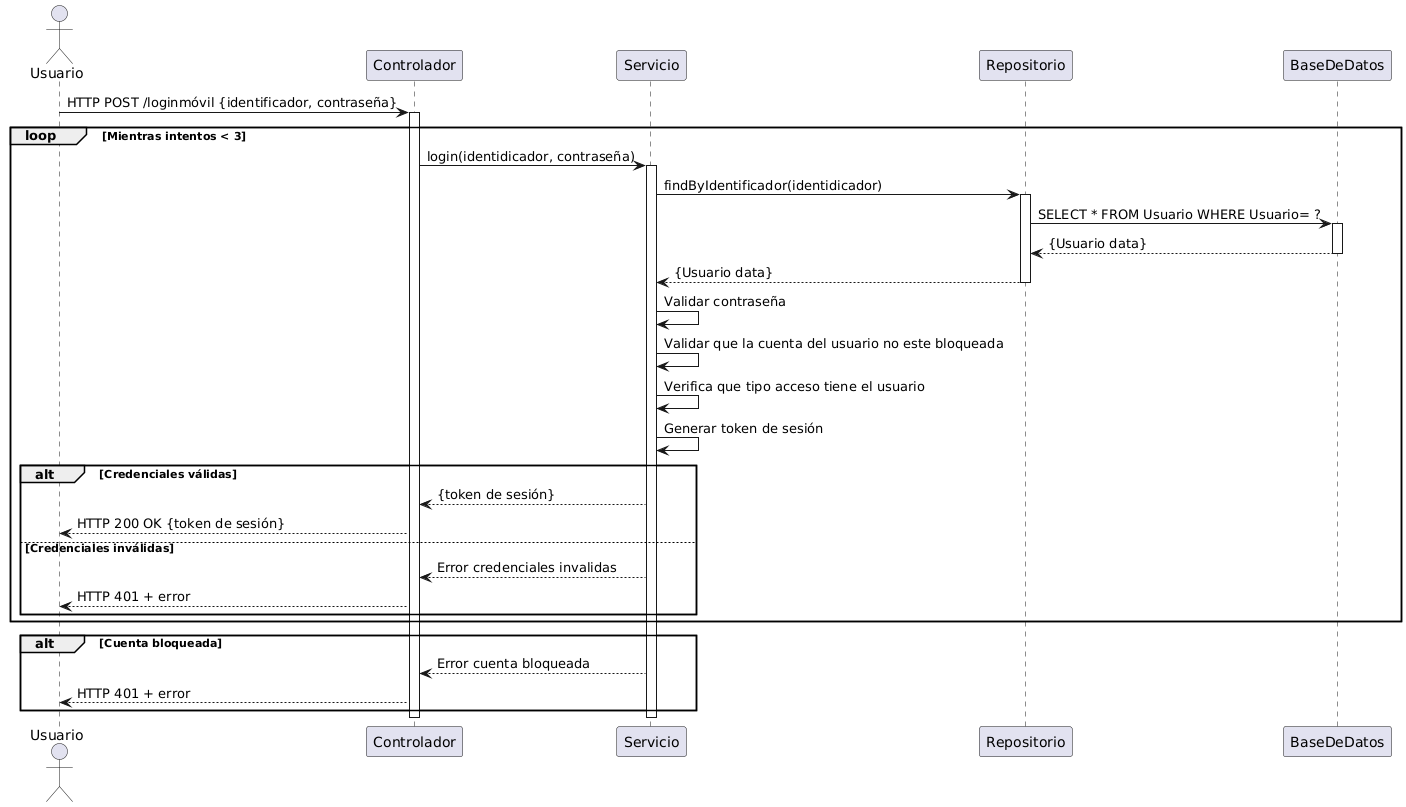
\includegraphics[width=1\textwidth]{Secuencia/CU-01.png}}
		\caption{Diagrama de secuencia del caso de uso número 01 (Iniciar sesión del sistema móvil).}
		\label{fig:Diagrama de secuencia CU-01}
	\end{center}
\end{figure}

En el diagrama de secuencia \ref{fig:Diagrama de secuencia CU-01} de secuencia se describe el proceso planeado para el caso de uso \hyperlink{CU-01}{CU-01 Iniciar sesión del sistema móvil}, mostrando las interacciones que tendrá con la vista, el controlador, el servicio, el repositorio y la base de datos.

\newpage

\subsection{SE-02 Consultar calendario escolar}

\begin{figure}[htbp!]
	\begin{center}
		\fbox{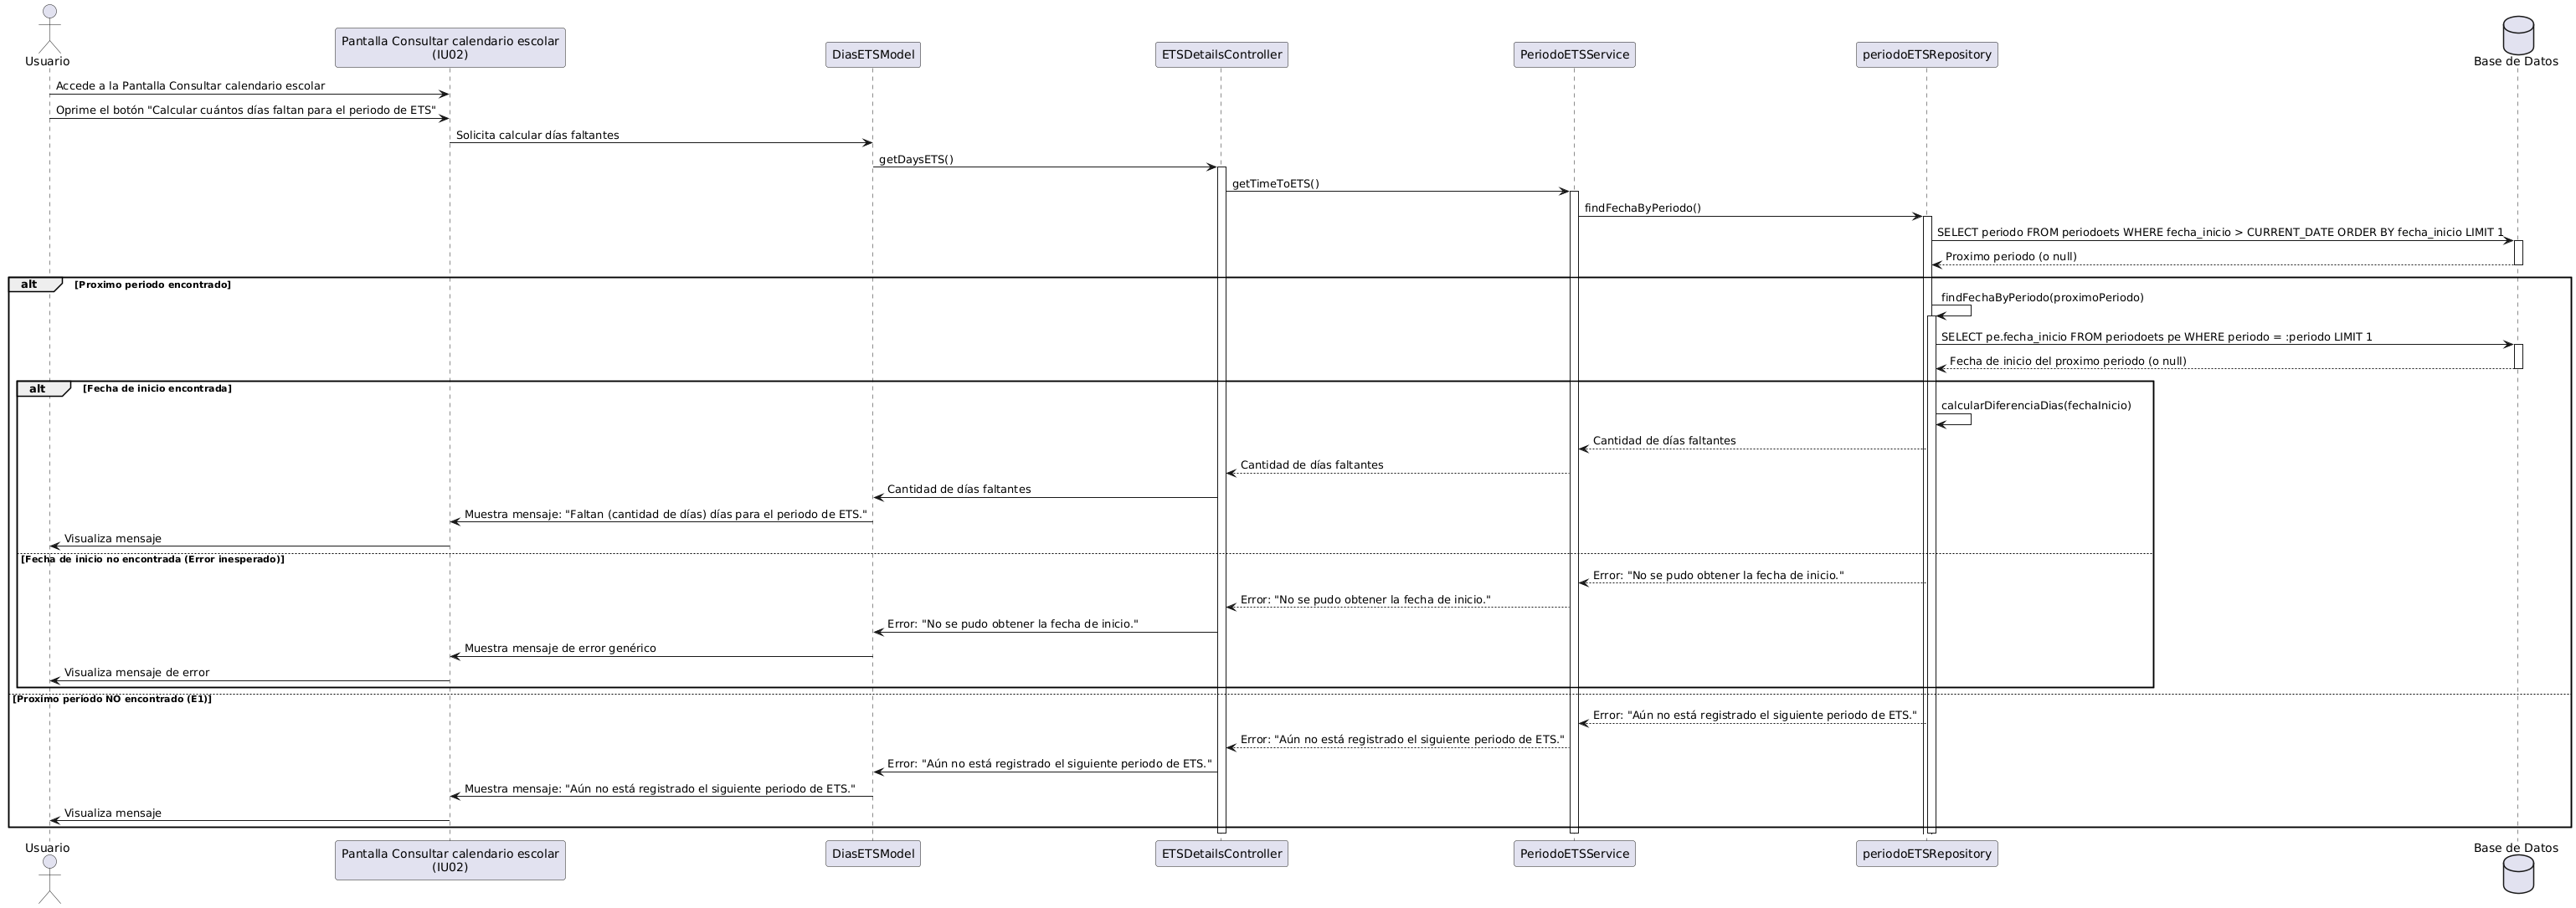
\includegraphics[width=1\textwidth]{Secuencia/CU-02.png}}
		\caption{Diagrama de secuencia del caso de uso número 02 (Consultar calendario escolar).}
		\label{fig:Diagrama de secuencia CU-02}
	\end{center}
\end{figure}

En el diagrama de secuencia \ref{fig:Diagrama de secuencia CU-02} se describe el proceso planeado para el caso de uso \hyperlink{CU-02}{CU-02 Consultar calendario escolar}, mostrando las interacciones que tendrá con la vista, el controlador, el servicio, el repositorio y la base de datos.

\newpage

\subsection{SE-03 Consultar notificaciones}

\begin{figure}[htbp!]
	\begin{center}
		\fbox{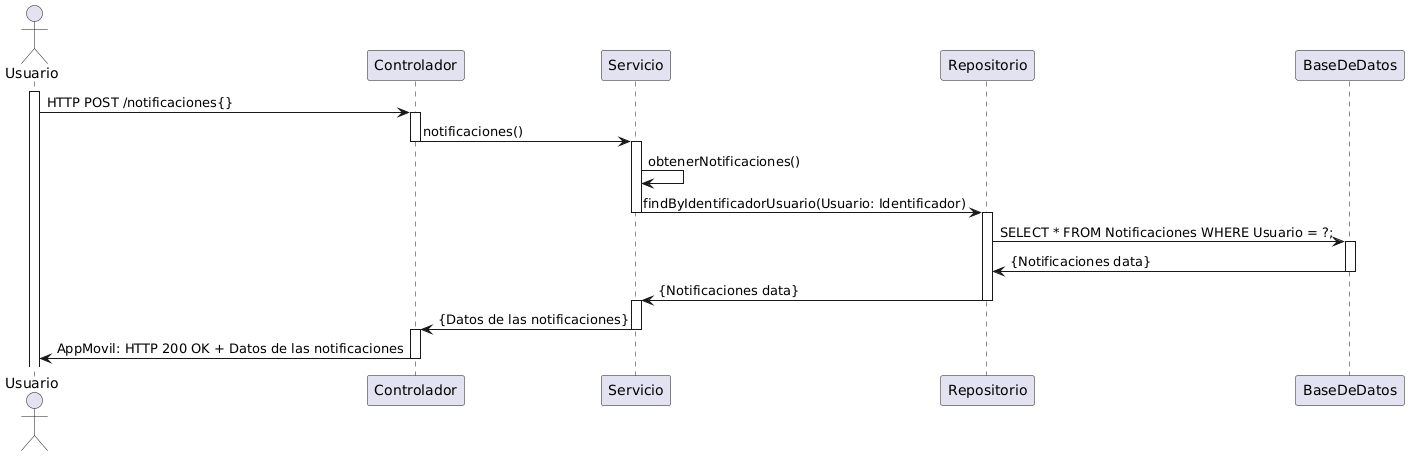
\includegraphics[width=1\textwidth]{Secuencia/CU-03.png}}
		\caption{Diagrama de secuencia del caso de uso número 03 (Consultar notificaciones).}
		\label{fig:Diagrama se secuencia CU-03}
	\end{center}
\end{figure}

En el diagrama de secuencia \ref{fig:Diagrama de secuencia CU-03} se describe el proceso planeado para el caso de uso \hyperlink{CU-03}{CU-03 Consultar notificaciones}, mostrando las interacciones que tendrá con la vista, el controlador, el servicio, el repositorio y la base de datos.

\newpage

\subsection{SE-04 Consultar periodos de ETS asignados al docente}

\begin{figure}[htbp!]
	\begin{center}
		\fbox{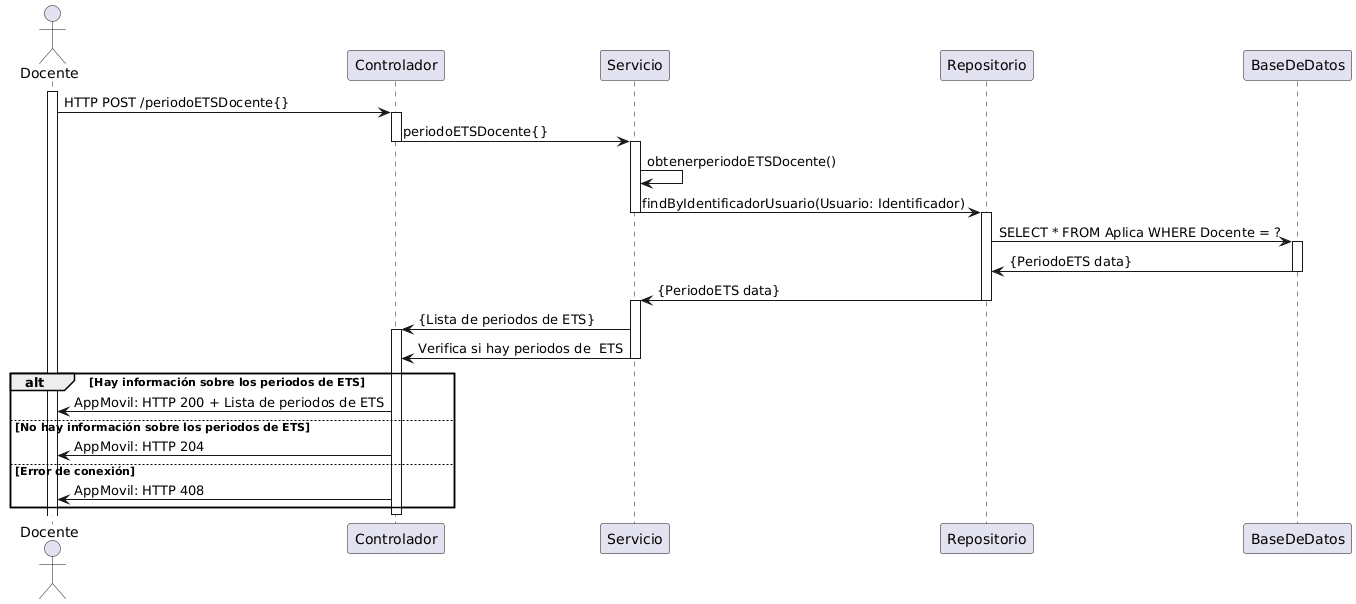
\includegraphics[width=1\textwidth]{Secuencia/CU-04.png}}
		\caption{Diagrama de secuencia del caso de uso número 04 (Consultar periodos de ETS asignados al docente).}
		\label{fig:Diagrama de secuencia CU-04}
	\end{center}
\end{figure}

En el diagrama de secuencia \ref{fig:Diagrama de secuencia CU-04} se describe el proceso planeado para el caso de uso \hyperlink{CU-04}{CU-04 Consultar periodos de ETS asignados al docente}, mostrando las interacciones que tendrá con la vista, el controlador, el servicio, el repositorio y la base de datos.

\newpage

\subsection{SE-05 Consultar ETS asignados}

\begin{figure}[htbp!]
	\begin{center}
		\fbox{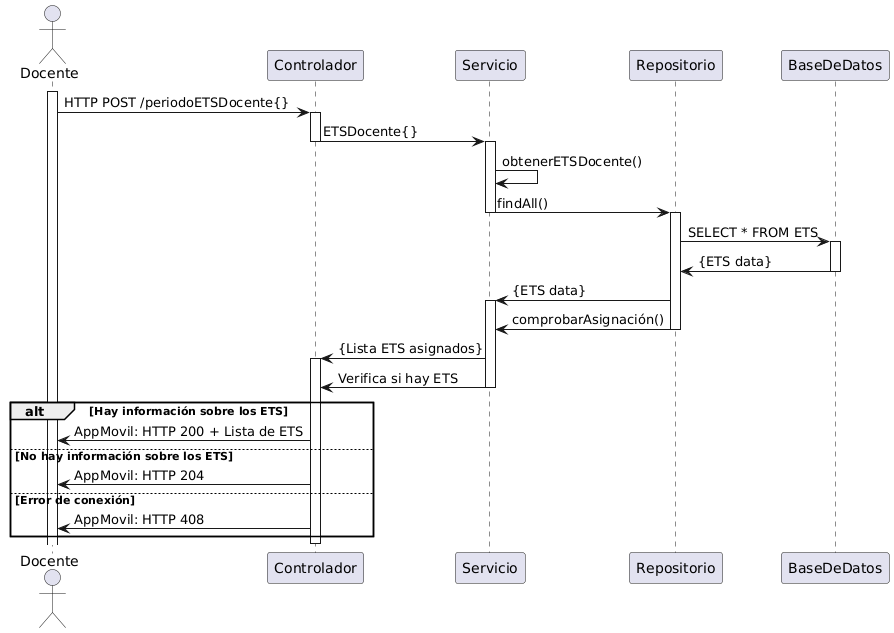
\includegraphics[width=1\textwidth]{Secuencia/CU-05.png}}
		\caption{Diagrama de secuencia del caso de uso número 05 (Consultar ETS asignados).}
		\label{fig:Diagrama de secuencia CU-05}
	\end{center}
\end{figure}

En el diagrama de secuencia \ref{fig:Diagrama de secuencia CU-05} se describe el proceso planeado para el caso de uso \hyperlink{CU-05}{CU-05 Consultar ETS asignados}, mostrando las interacciones que tendrá con la vista, el controlador, el servicio, el repositorio y la base de datos.

\newpage

\subsection{SE-06 Mostrar información de los ETS asignados}

\begin{figure}[htbp!]
	\begin{center}
		\fbox{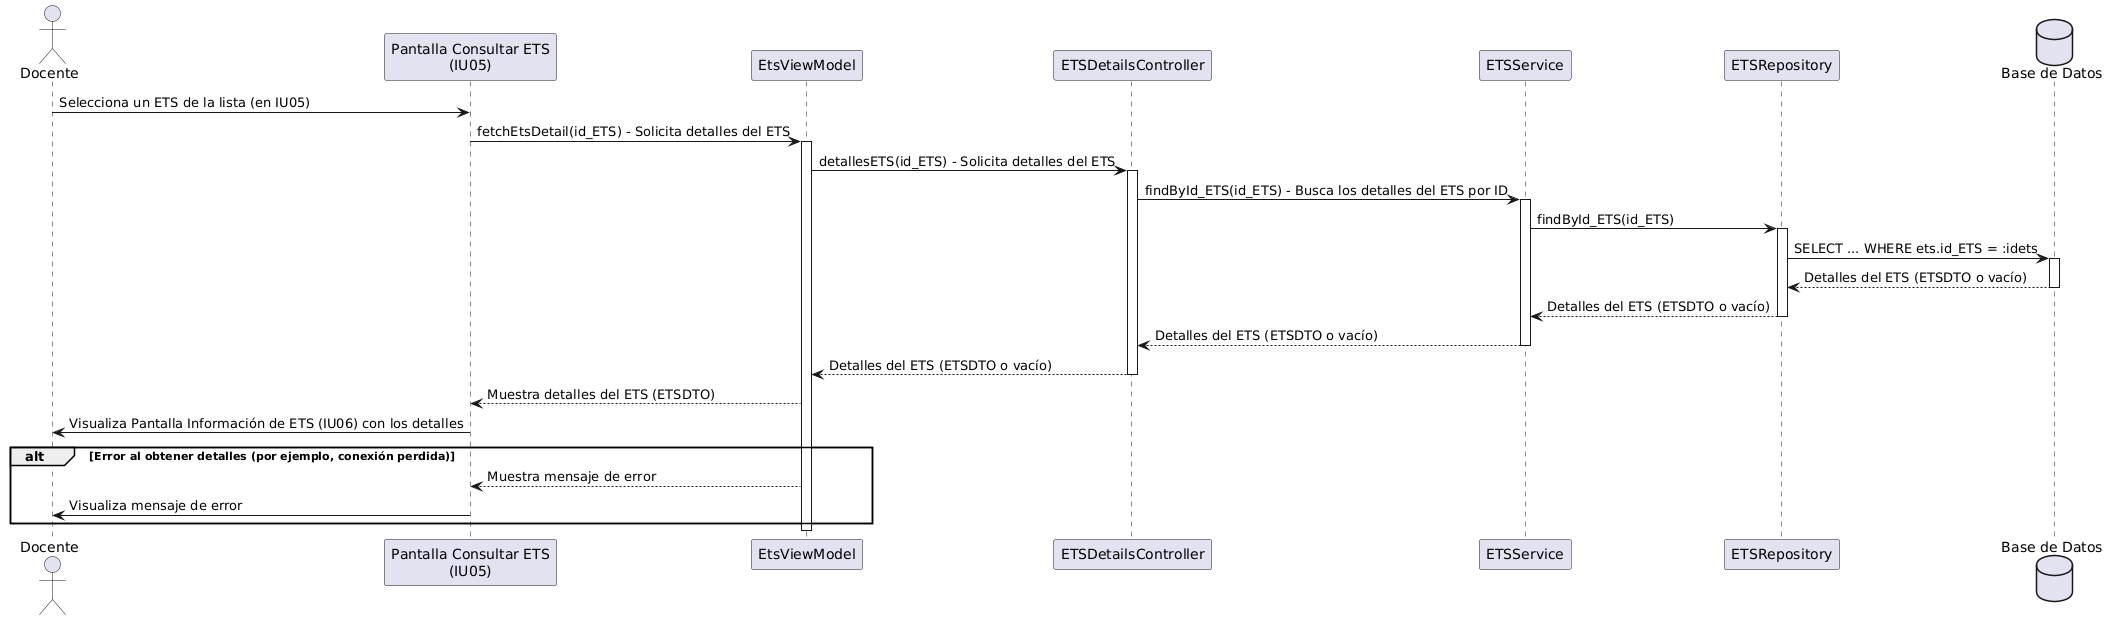
\includegraphics[width=1\textwidth]{Secuencia/CU-06.png}}
		\caption{Diagrama de secuencia del caso de uso número 06 (Mostrar información de los ETS asignados).}
		\label{fig:Diagrama de secuencia CU-06}
	\end{center}
\end{figure}

En el diagrama de secuencia \ref{fig:Diagrama de secuencia CU-06} se describe el proceso planeado para el caso de uso \hyperlink{CU-06}{CU-06 Mostrar información de los ETS asignados}, mostrando las interacciones que tendrá con la vista, el controlador, el servicio, el repositorio y la base de datos.

\newpage

\subsection{SE-07 Solicitar remplazo}

\begin{figure}[htbp!]
	\begin{center}
		\fbox{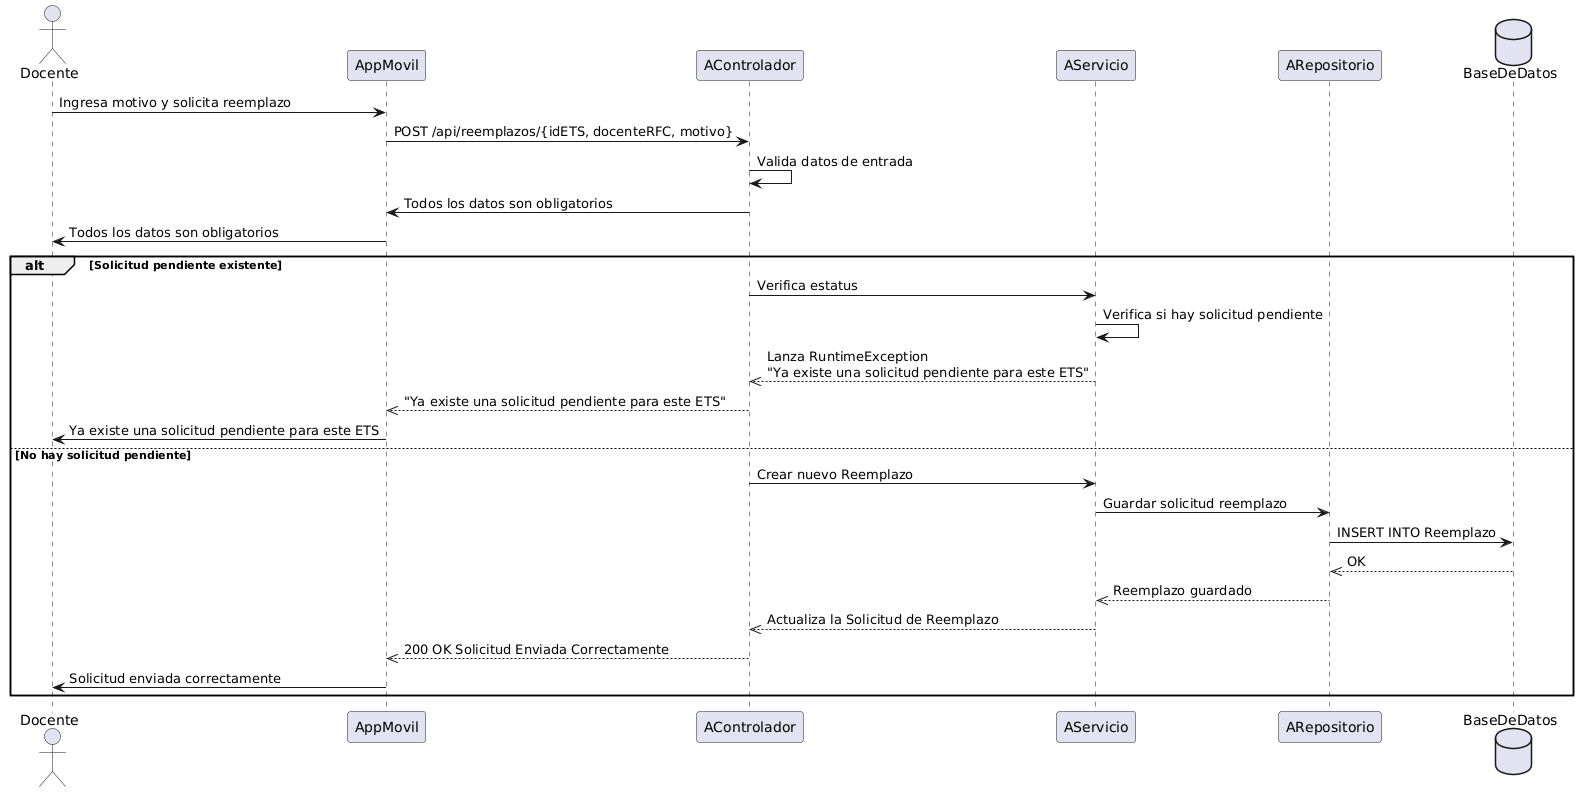
\includegraphics[width=1\textwidth]{Secuencia/CU-07.png}}
		\caption{Diagrama de secuencia del caso de uso número 07 (Solicitar remplazo).}
		\label{fig:Diagrama de secuencia CU-07}
	\end{center}
\end{figure}

En el diagrama de secuencia \ref{fig:Diagrama de secuencia CU-07} se describe el proceso planeado para el caso de uso \hyperlink{CU-07}{CU-07 Solicitar remplazo}, mostrando las interacciones que tendrá con la vista, el controlador, el servicio, el repositorio y la base de datos.

\newpage

\subsection{SE-08 Consultar lista de alumnos inscritos a un ETS}

\begin{figure}[htbp!]
	\begin{center}
		\fbox{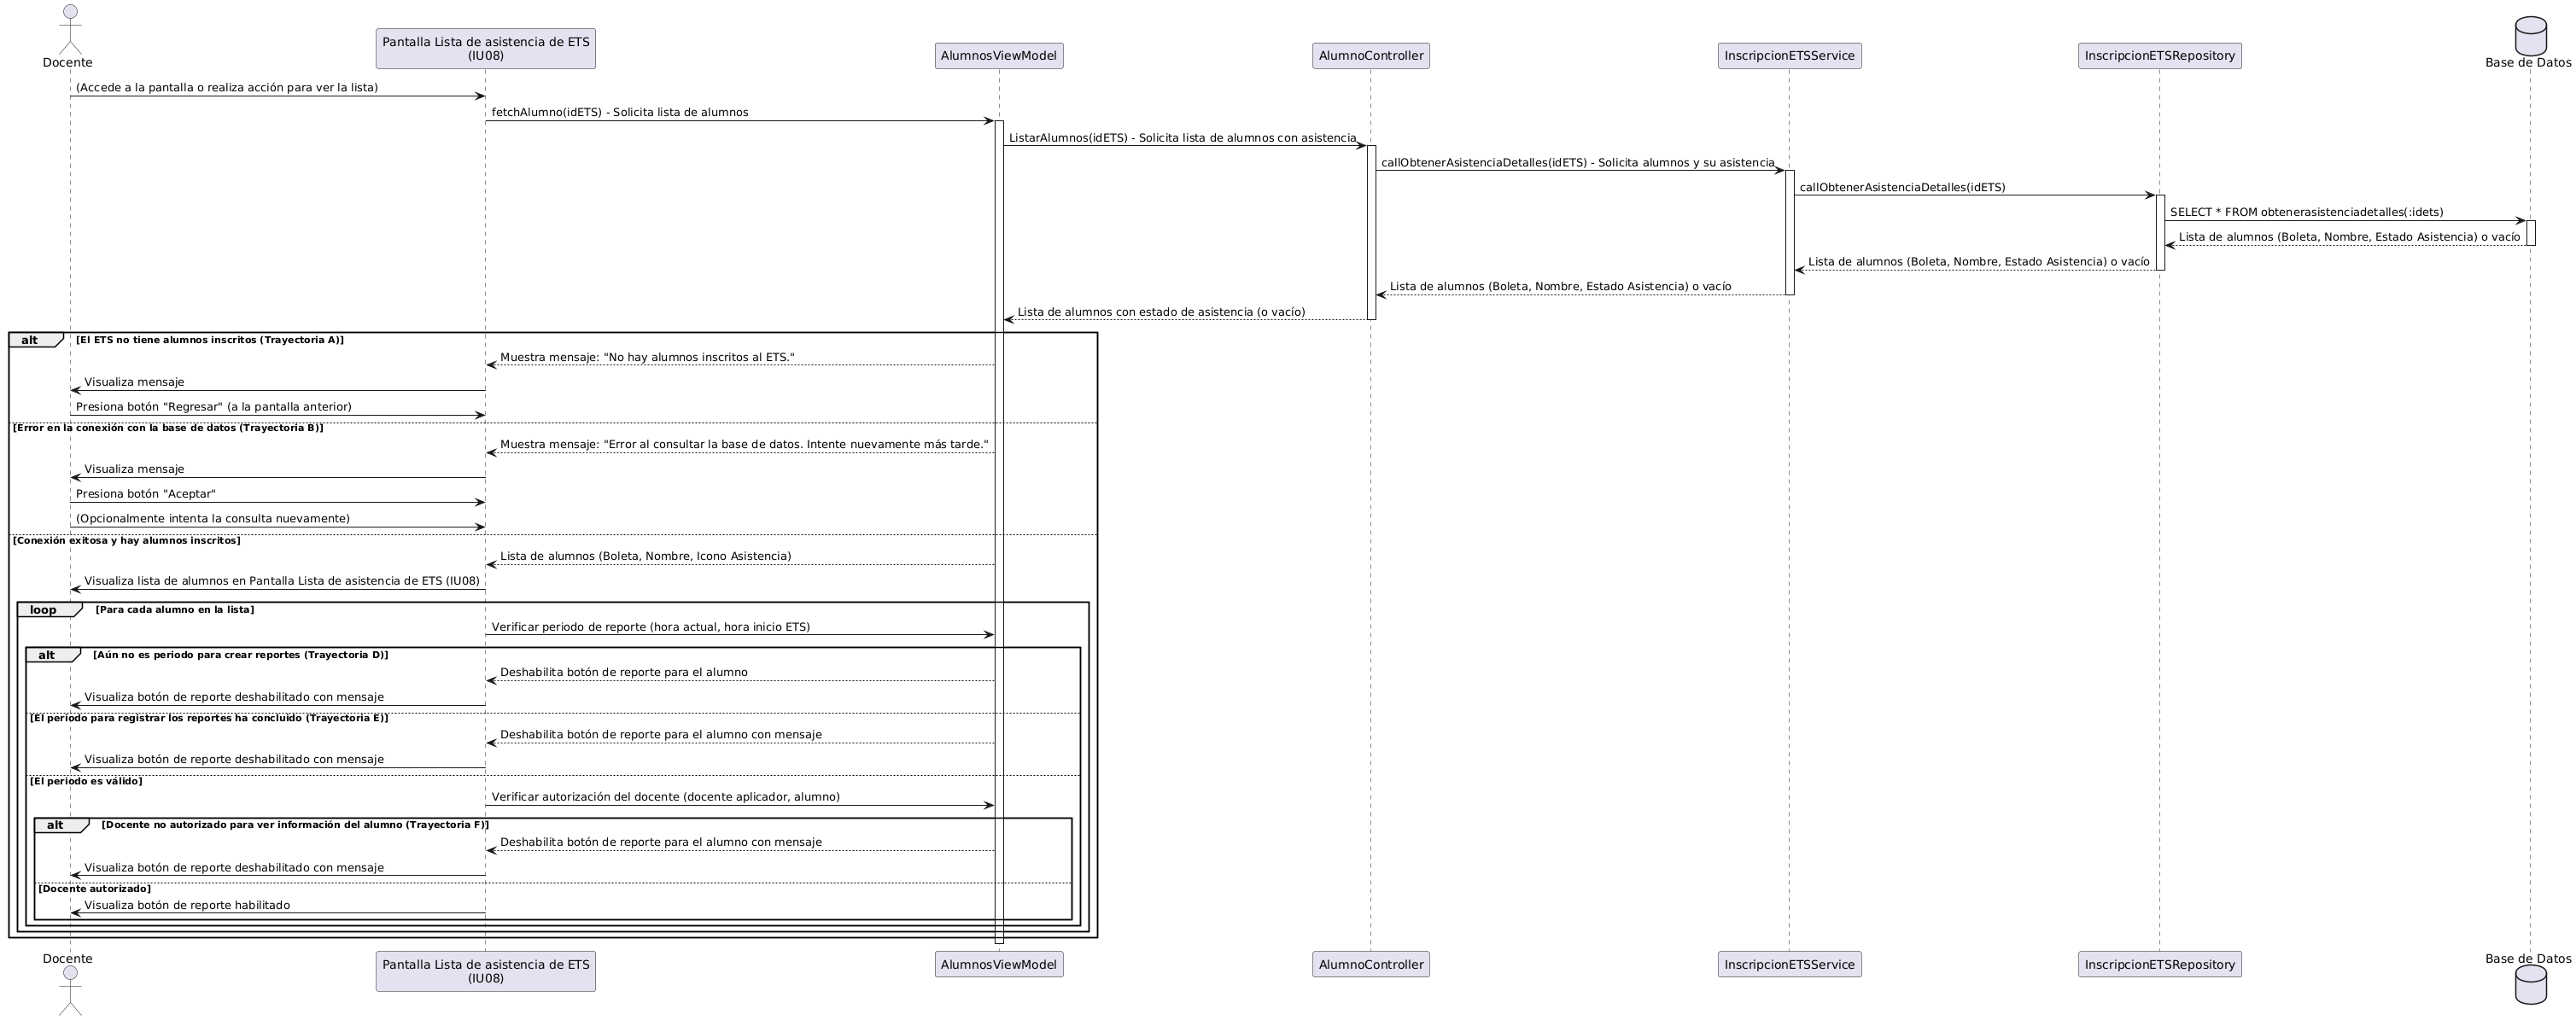
\includegraphics[width=1\textwidth]{Secuencia/CU-08.png}}
		\caption{Diagrama de secuencia del caso de uso número 08 (Consultar lista de alumnos inscritos a un ETS).}
		\label{fig:Diagrama de secuencia CU-08}
	\end{center}
\end{figure}

En el diagrama de secuencia \ref{fig:Diagrama de secuencia CU-08} se describe el proceso planeado para el caso de uso \hyperlink{CU-08}{CU-08 Consultar lista de alumnos inscritos a un ETS}, mostrando las interacciones que tendrá con la vista, el controlador, el servicio, el repositorio y la base de datos.

\newpage

\subsection{SE-09 Tomar asistencias a los ETS}

\begin{figure}[htbp!]
	\begin{center}
		\fbox{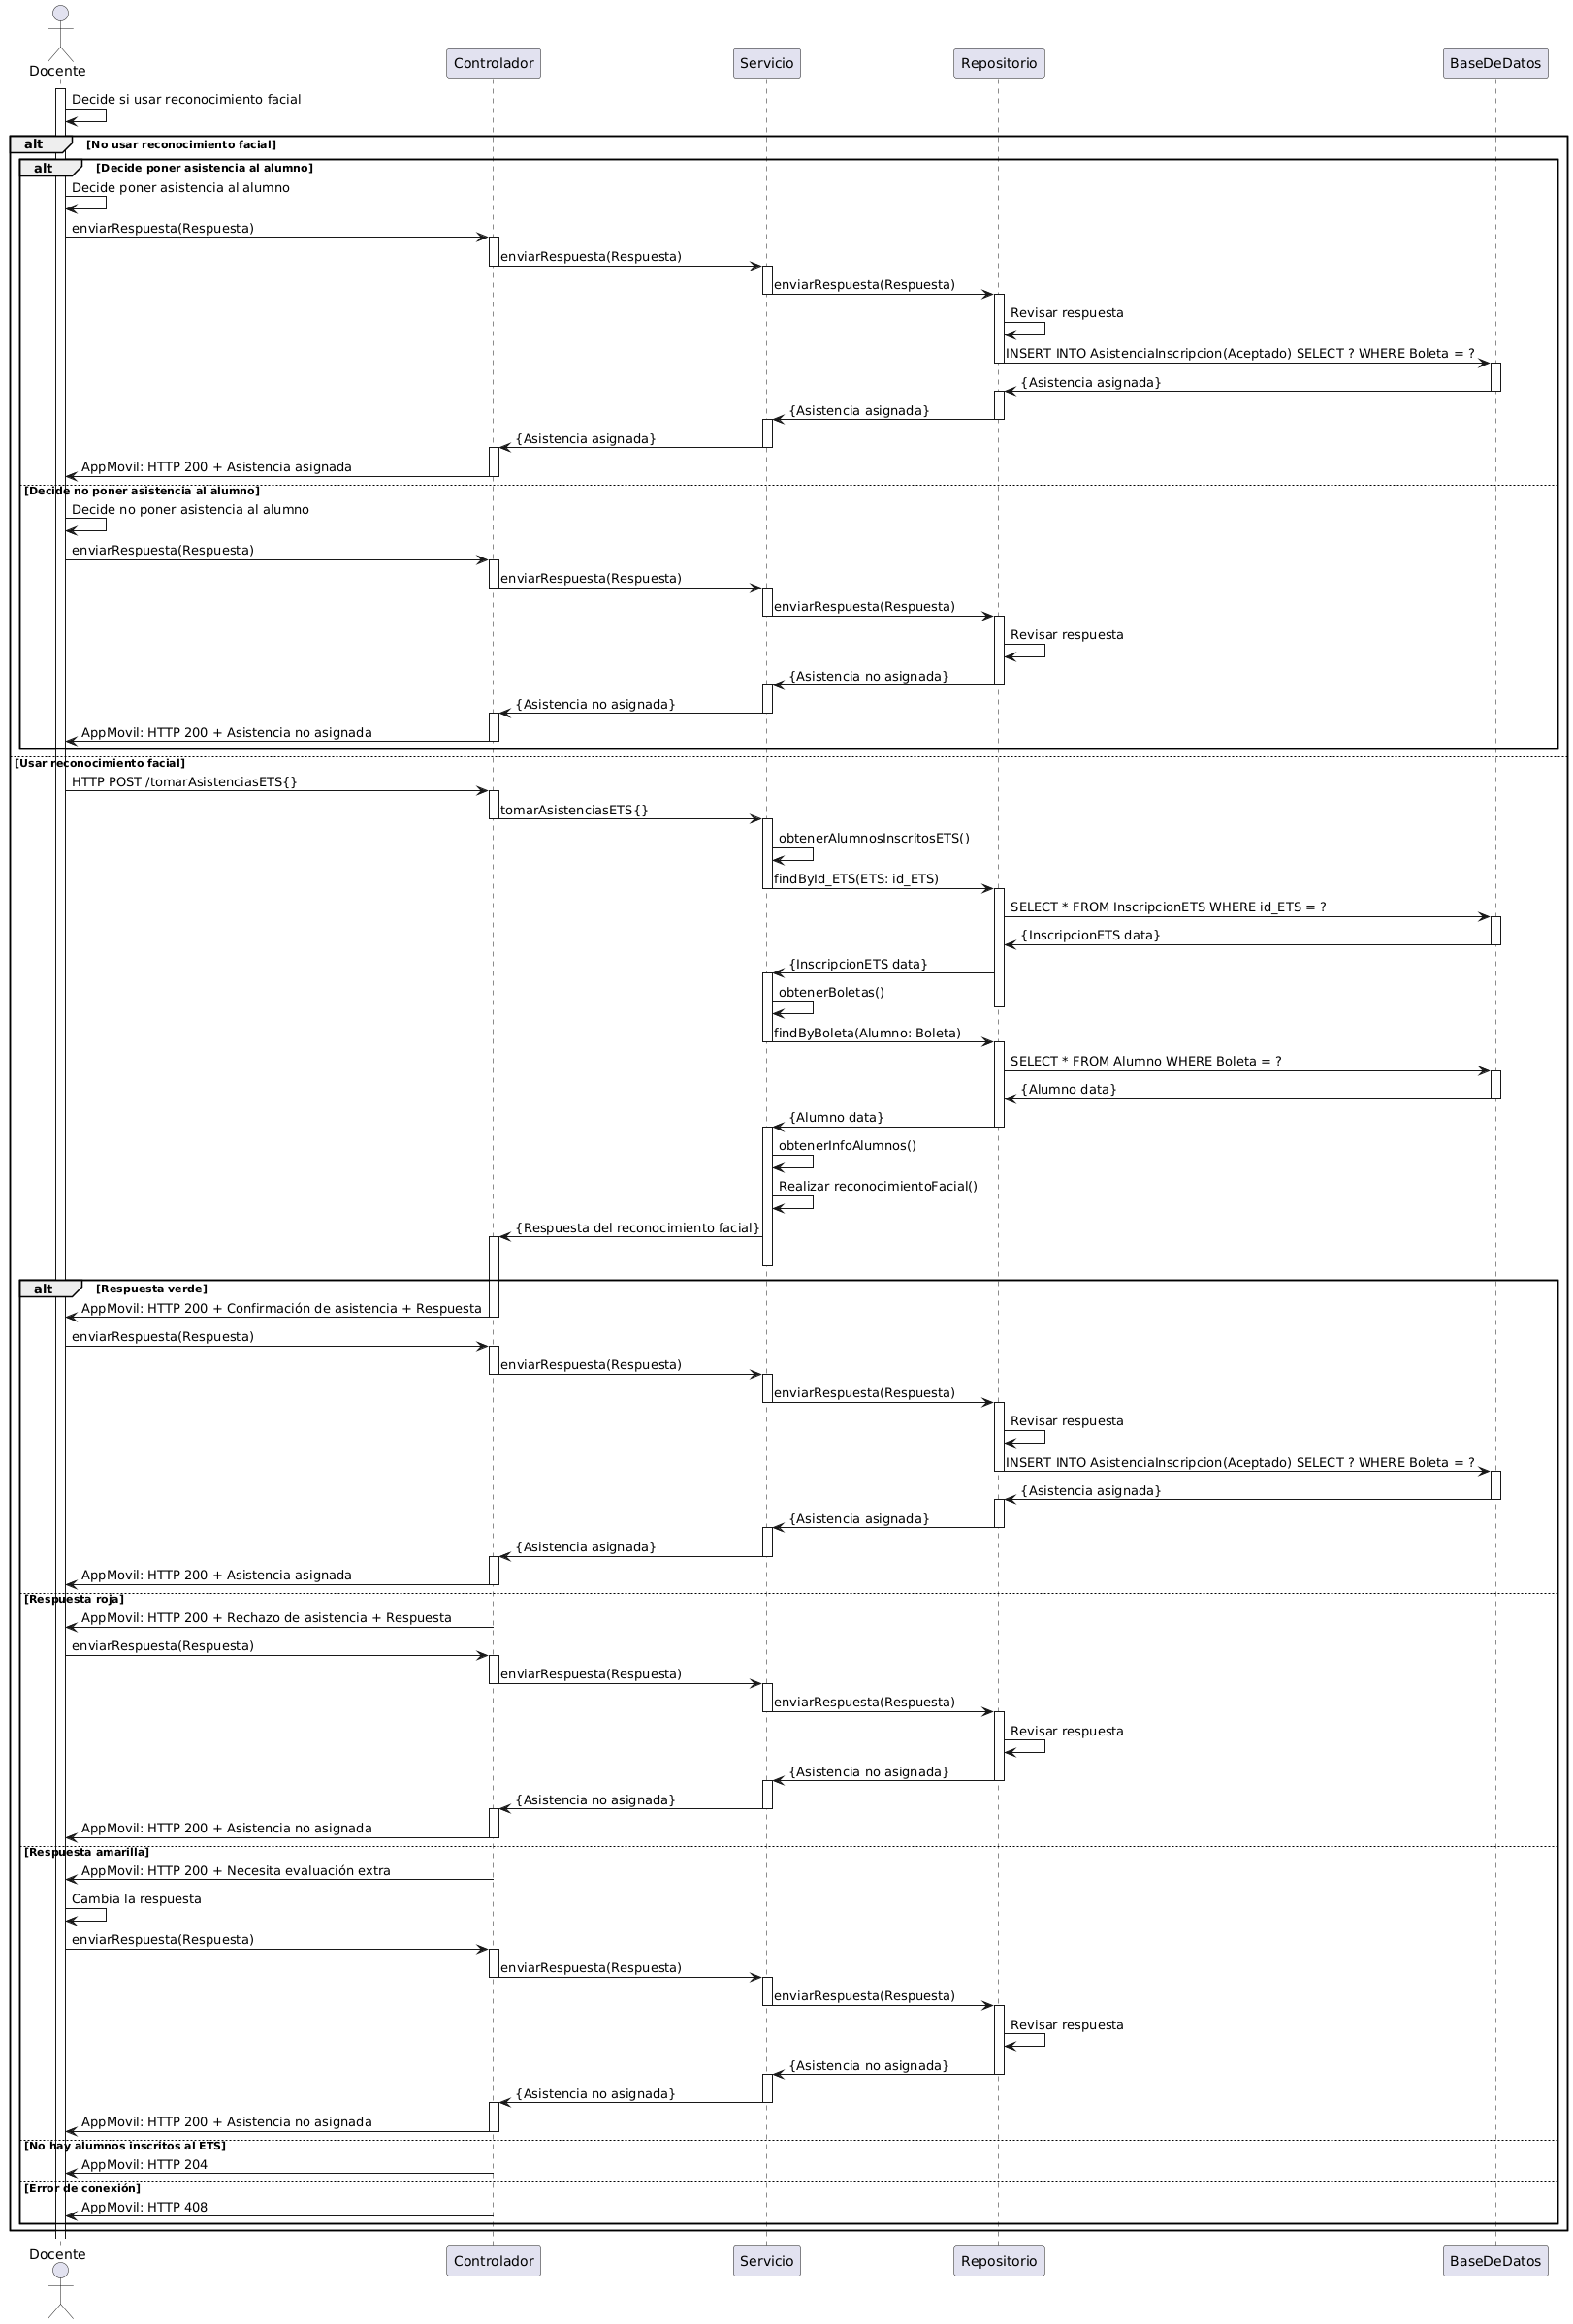
\includegraphics[width=.7\textwidth]{Secuencia/CU-09.png}}
		\caption{Diagrama de secuencia del caso de uso número 09 (Tomar asistencias a los ETS).}
		\label{fig:Diagrama de secuencia CU-09}
	\end{center}
\end{figure}

En el diagrama de secuencia \ref{fig:Diagrama de secuencia CU-09} se describe el proceso planeado para el caso de uso \hyperlink{CU-09}{CU-09 Tomar asistencias a los ETS}, mostrando las interacciones que tendrá con la vista, el controlador, el servicio, el repositorio y la base de datos.

\subsection{SE-10 Consultar lista de asistencia de alumnos inscritos a los ETS}

\begin{figure}[htbp!]
	\begin{center}
		\fbox{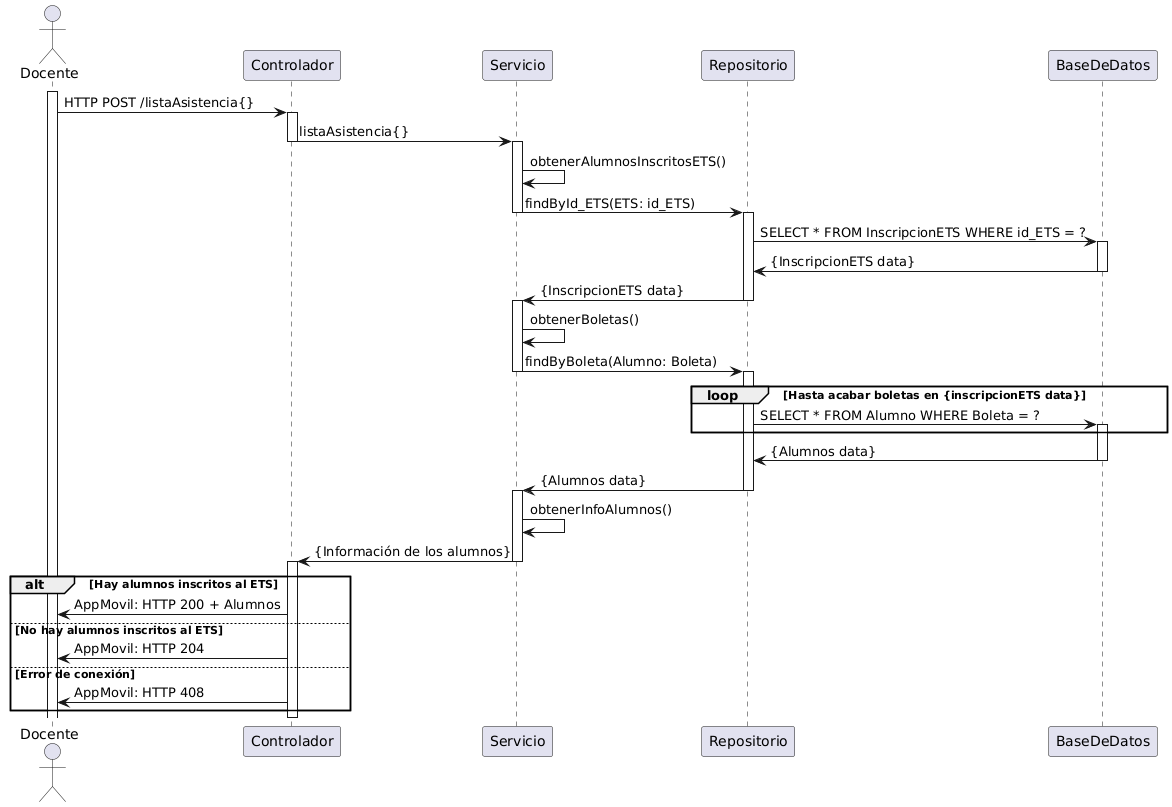
\includegraphics[width=1\textwidth]{Secuencia/CU-10.png}}
		\caption{Diagrama de secuencia del caso de uso número 10 (Consultar lista de asistencia de alumnos inscritos a los ETS).}
		\label{fig:Diagrama de secuencia CU-10}
	\end{center}
\end{figure}

En el diagrama de secuencia \ref{fig:Diagrama de secuencia CU-10} se describe el proceso planeado para el caso de uso \hyperlink{CU-10}{CU-10 Consultar lista de asistencia de alumnos inscritos a los ETS}, mostrando las interacciones que tendrá con la vista, el controlador, el servicio, el repositorio y la base de datos.

\newpage

\subsection{SE-11 Mostrar la foto e información  del alumno}

\begin{figure}[htbp!]
	\begin{center}
		\fbox{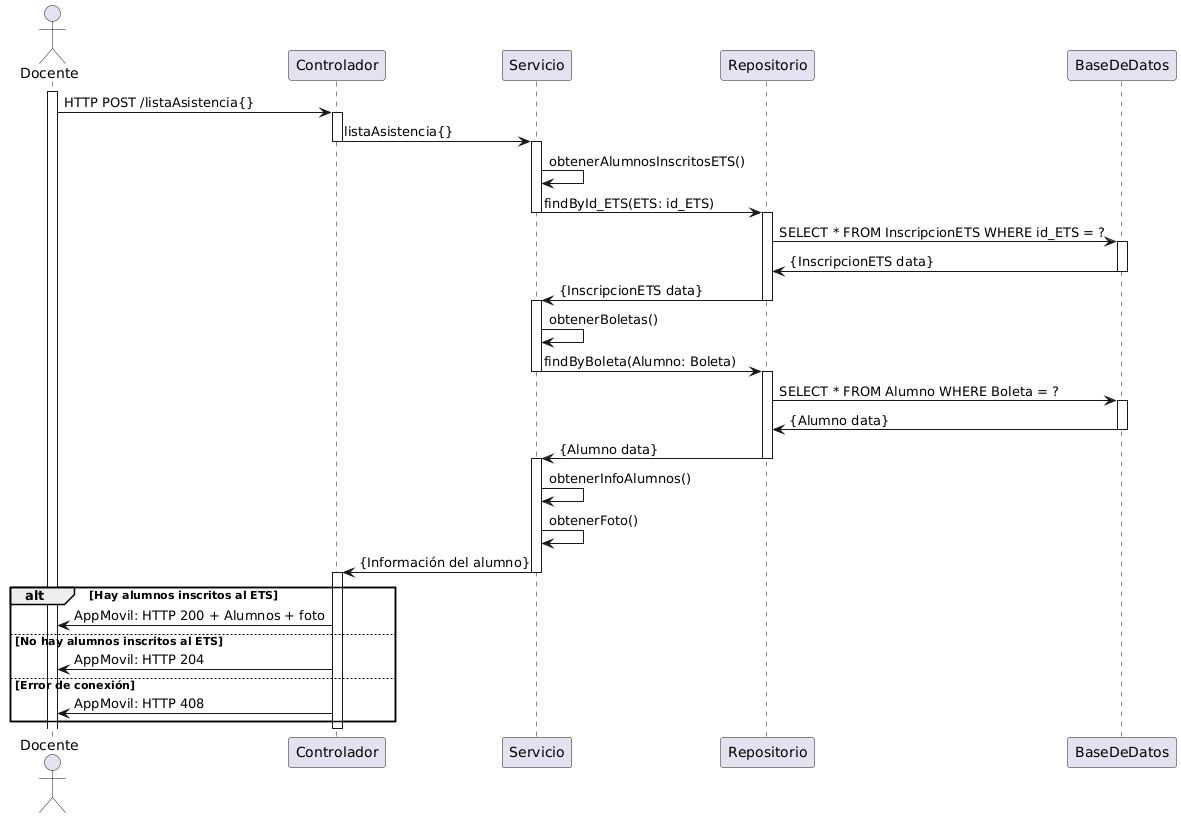
\includegraphics[width=1\textwidth]{Secuencia/CU-11.png}}
		\caption{Diagrama de secuencia del caso de uso número 11 (Mostrar la foto e información  del alumno).}
		\label{fig:Diagrama de secuencia CU-11}
	\end{center}
\end{figure}


En el diagrama de secuencia \ref{fig:Diagrama de secuencia CU-11} se describe el proceso planeado para el caso de uso \hyperlink{CU-11}{CU-11 Mostrar la foto e información  del alumno}, mostrando las interacciones que tendrá con la vista, el controlador, el servicio, el repositorio y la base de datos.

\newpage

\subsection{SE-12 Consultar alumno mediante código QR de la credencial}

\begin{figure}[htbp!]
	\begin{center}
		\fbox{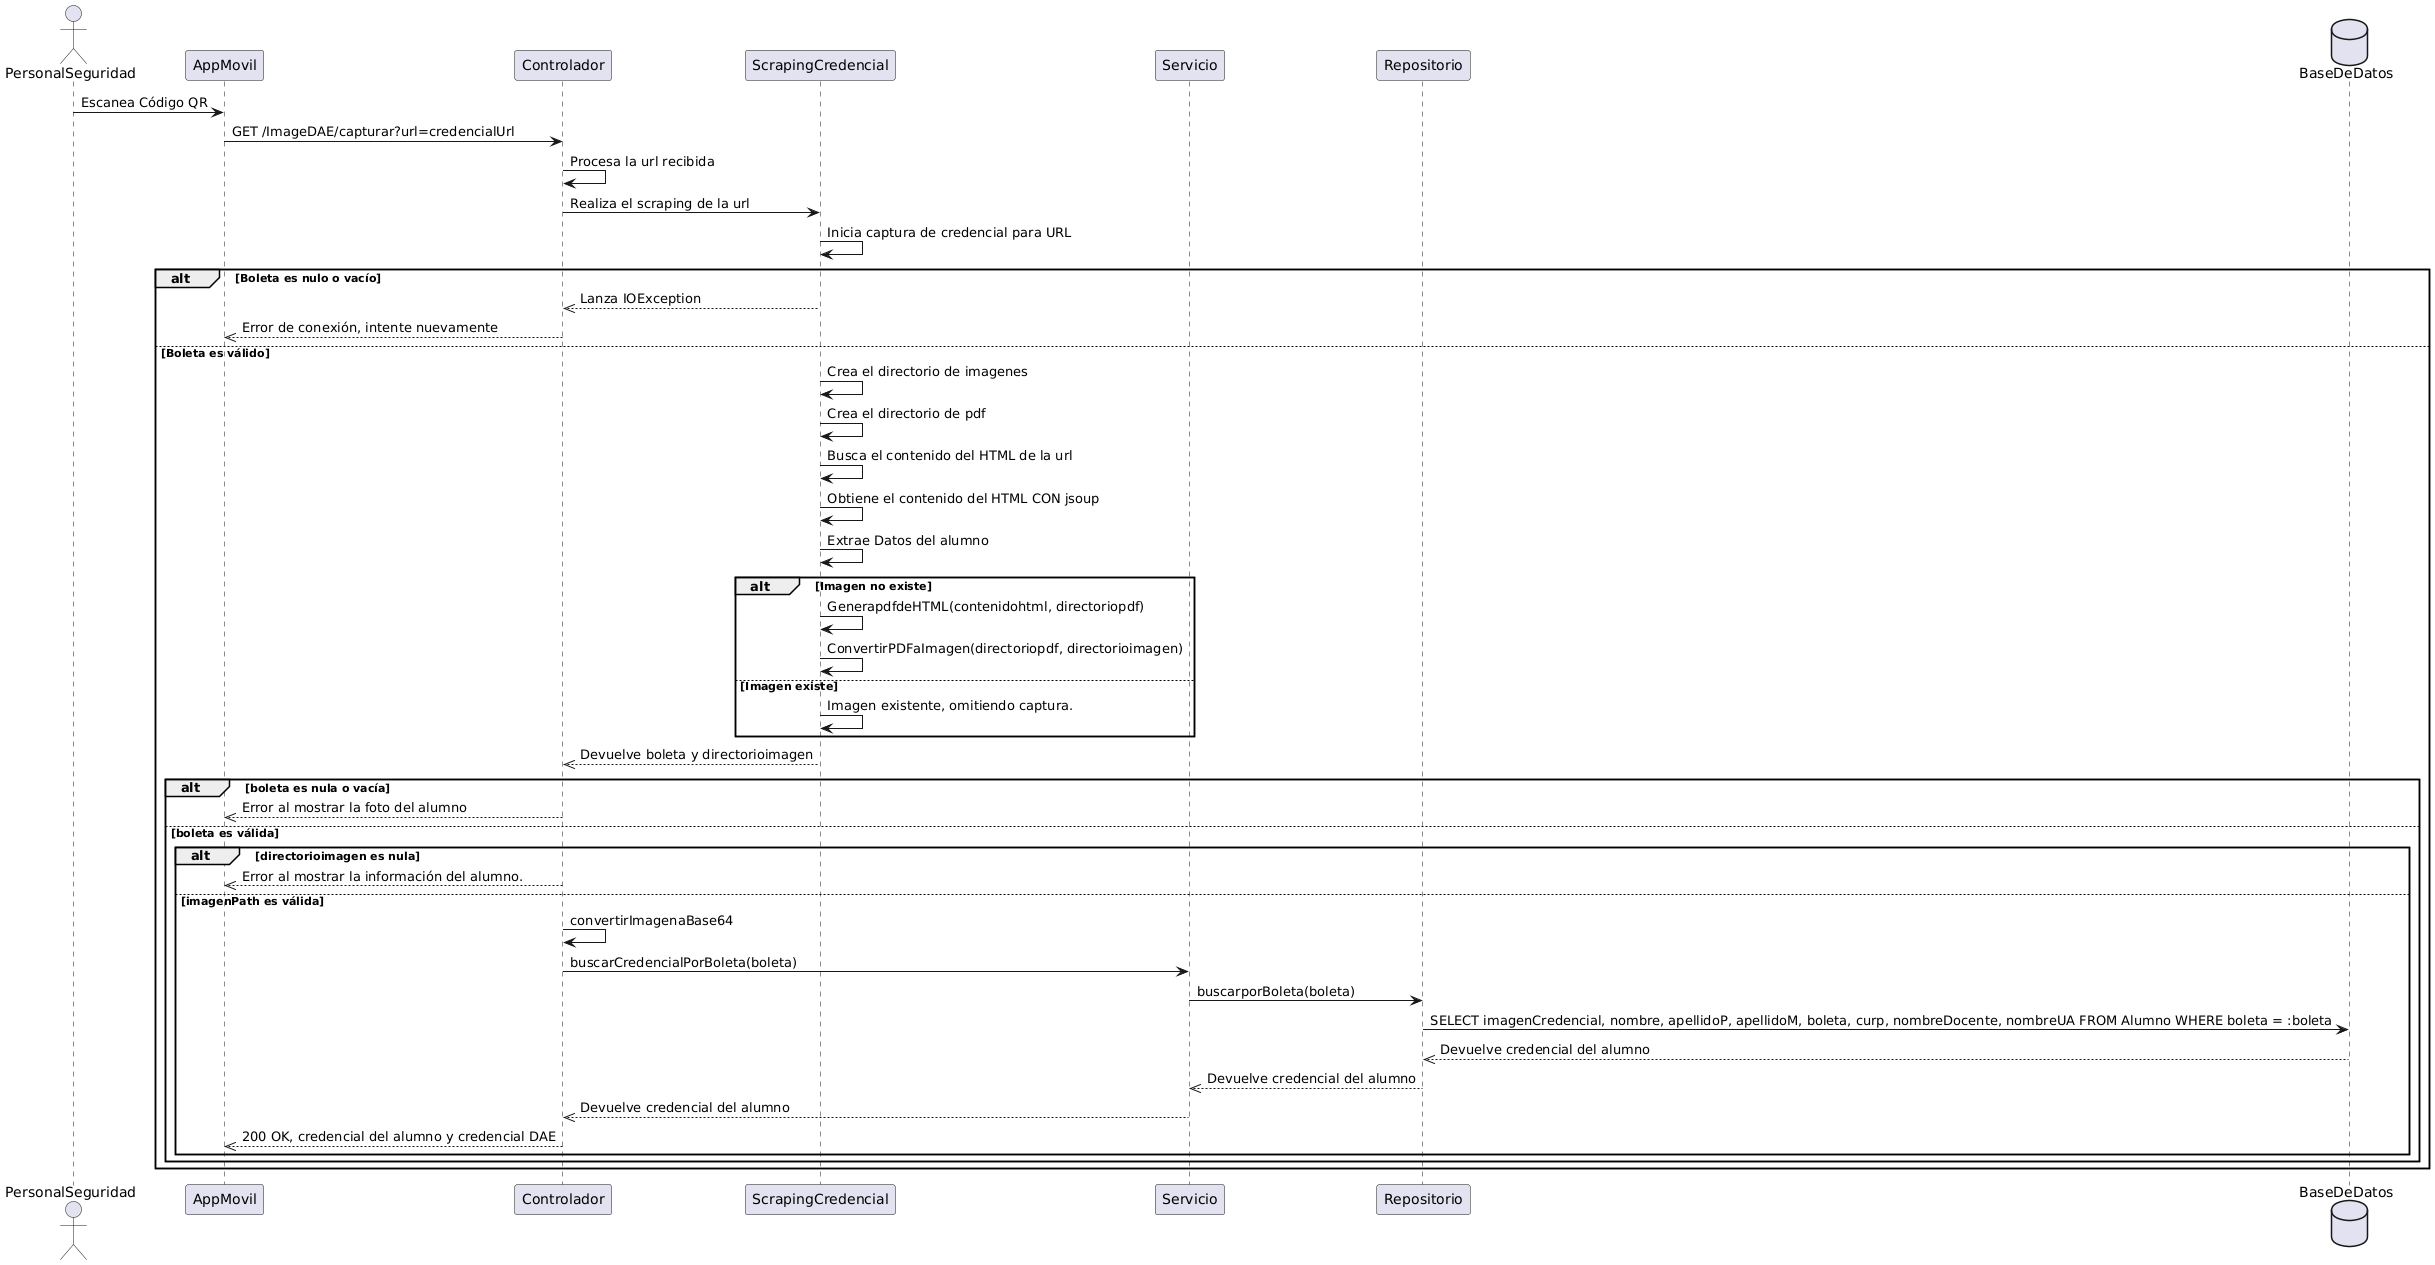
\includegraphics[width=1\textwidth]{Secuencia/CU-12.png}}
		\caption{Diagrama de secuencia del caso de uso número 12 (Consultar alumno mediante código QR de la credencial).}
		\label{fig:Diagrama de secuencia CU-12}
	\end{center}
\end{figure}

En el diagrama de secuencia \ref{fig:Diagrama de secuencia CU-12} se describe el proceso planeado para el caso de uso \hyperlink{CU-12}{CU-12 Consultar alumno mediante código QR de la credencial}, mostrando las interacciones que tendrá con la vista, el controlador, el servicio, el repositorio y la base de datos.

\newpage

\subsection{SE-13 Buscar alumno por boleta}

\begin{figure}[htbp!]
	\begin{center}
		\fbox{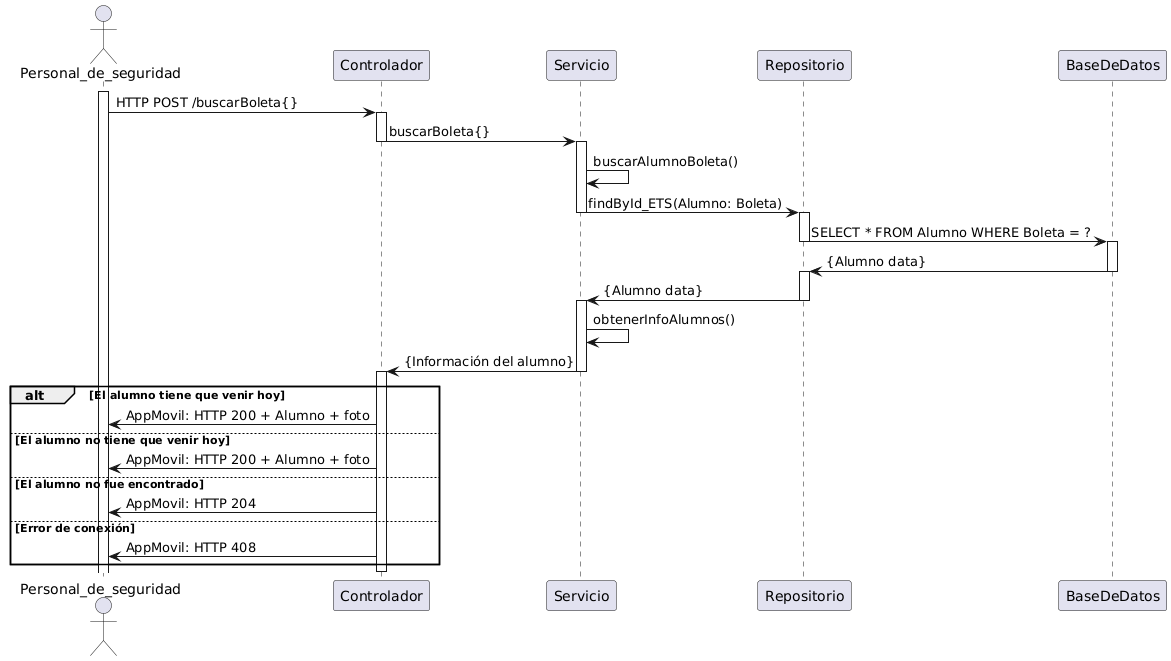
\includegraphics[width=1\textwidth]{Secuencia/CU-13.png}}
		\caption{Diagrama de secuencia del caso de uso número 13 (Buscar alumno por boleta).}
		\label{fig:Diagrama de secuencia CU-13}
	\end{center}
\end{figure}

En el diagrama de secuencia \ref{fig:Diagrama de secuencia CU-13} se describe el proceso planeado para el caso de uso \hyperlink{CU-13}{CU-13 Buscar alumno por boleta}, mostrando las interacciones que tendrá con la vista, el controlador, el servicio, el repositorio y la base de datos.

\newpage

\subsection{SE-14 Buscar alumno por nombre}

\begin{figure}[htbp!]
	\begin{center}
		\fbox{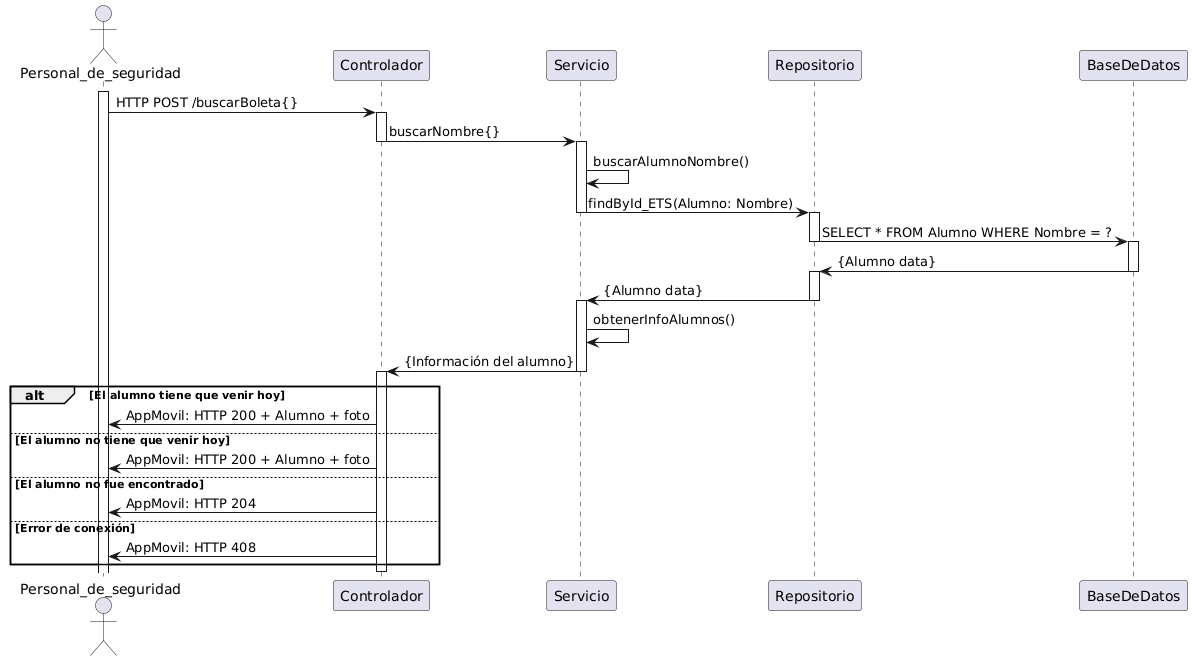
\includegraphics[width=1\textwidth]{Secuencia/CU-14.png}}
		\caption{Diagrama de secuencia del caso de uso número 14 (Buscar alumno por nombre).}
		\label{fig:Diagrama de secuencia CU-14}
	\end{center}
\end{figure}

En el diagrama de secuencia \ref{fig:Diagrama de secuencia CU-14} se describe el proceso planeado para el caso de uso \hyperlink{CU-14}{CU-14 Buscar alumno por nombre}, mostrando las interacciones que tendrá con la vista, el controlador, el servicio, el repositorio y la base de datos.

\newpage

\subsection{SE-15 Registrar asistencia}

\begin{figure}[htbp!]
	\begin{center}
		\fbox{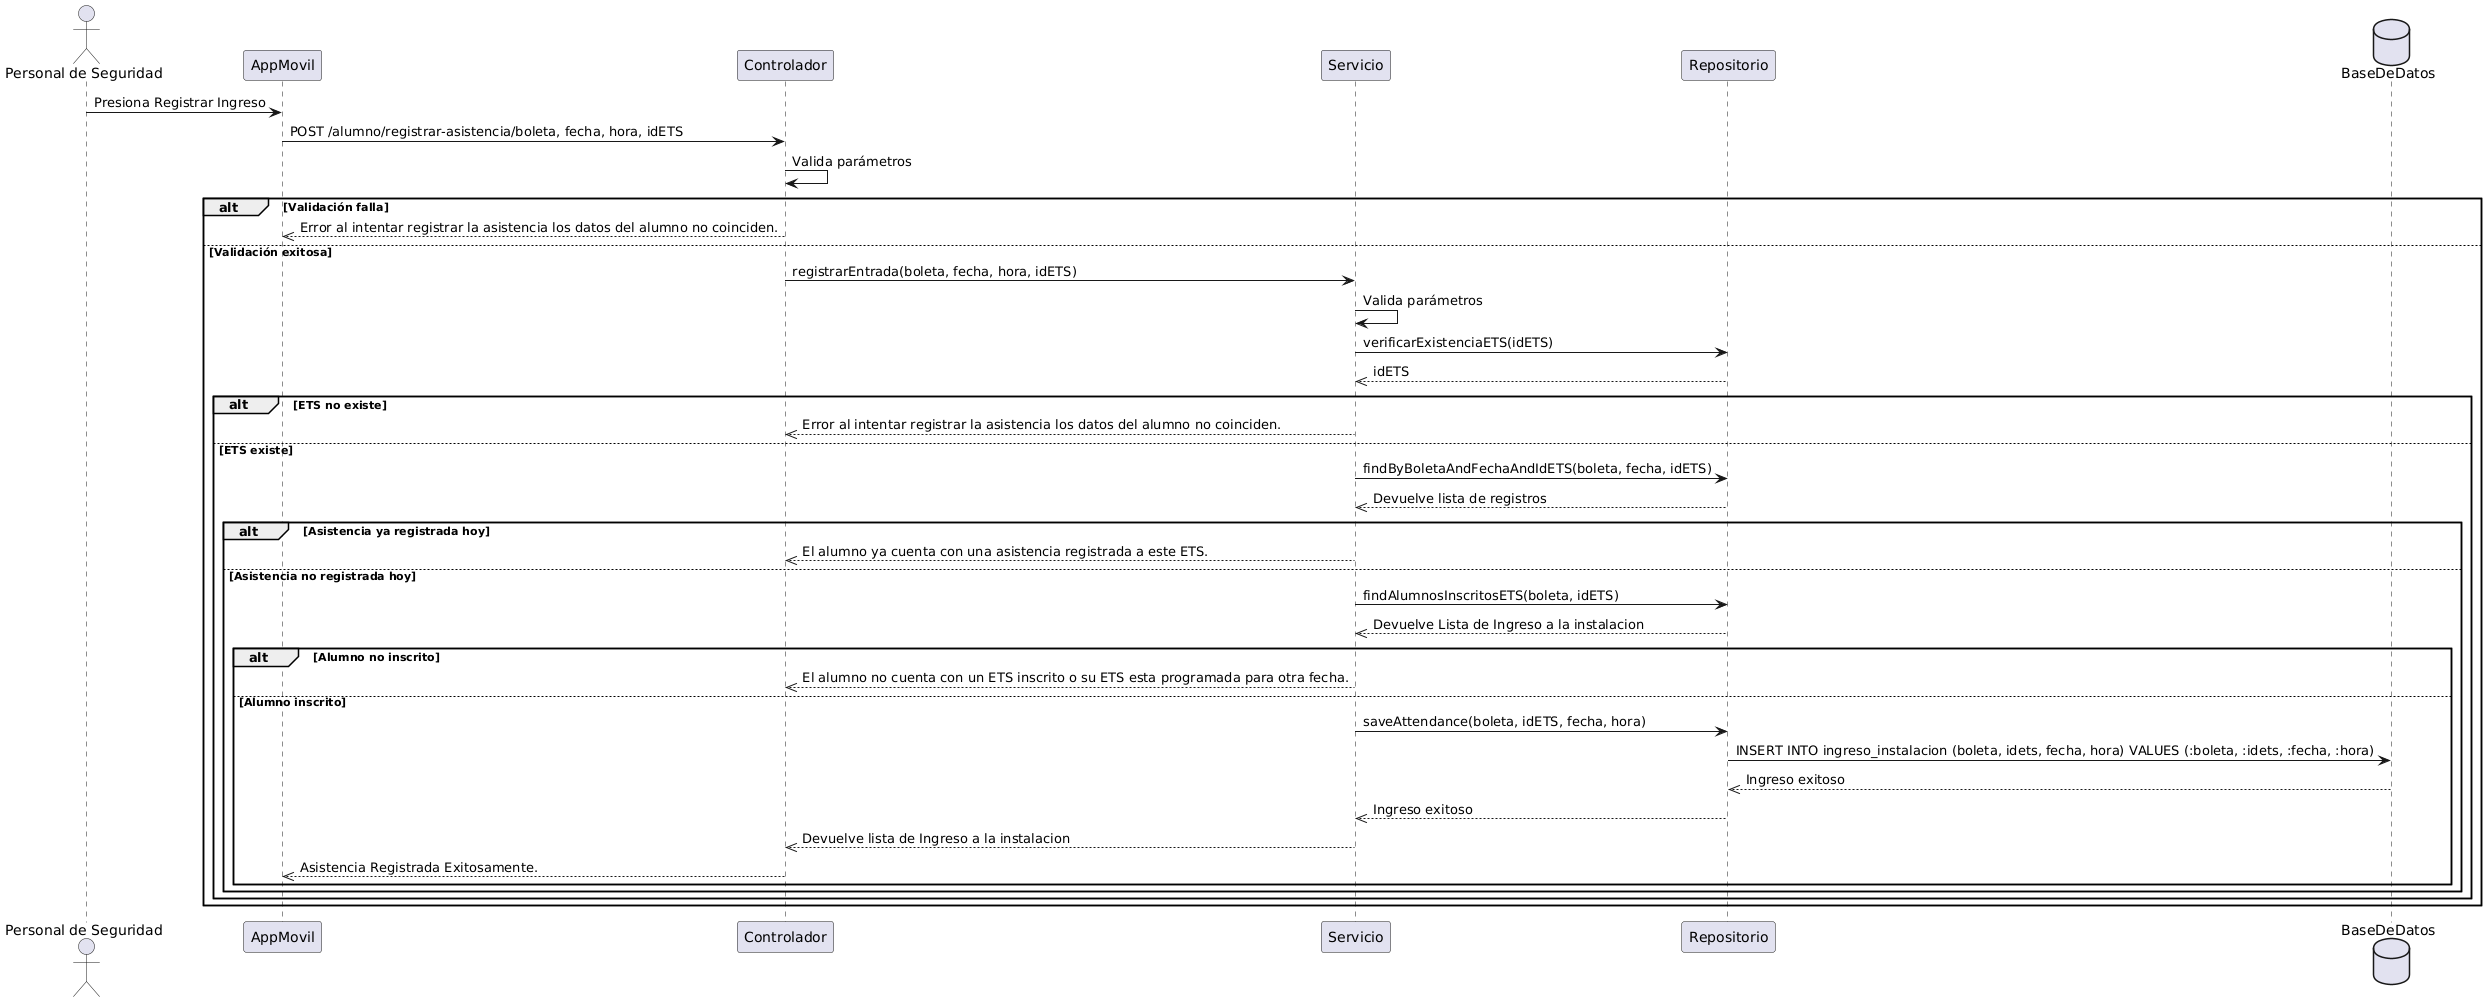
\includegraphics[width=.7\textwidth]{Secuencia/CU-15.png}}
		\caption{Diagrama de secuencia del caso de uso número 15 (Registrar asistencia).}
		\label{fig:Diagrama de secuencia CU-15}
	\end{center}
\end{figure}

En el diagrama de secuencia \ref{fig:Diagrama de secuencia CU-15} se describe el proceso planeado para el caso de uso \hyperlink{CU-15}{CU-15 Registrar asistencia}, mostrando las interacciones que tendrá con la vista, el controlador, el servicio, el repositorio y la base de datos.

\subsection{SE-16 Consultar periodos de ETS inscritos del alumno}

\begin{figure}[htbp!]
	\begin{center}
		\fbox{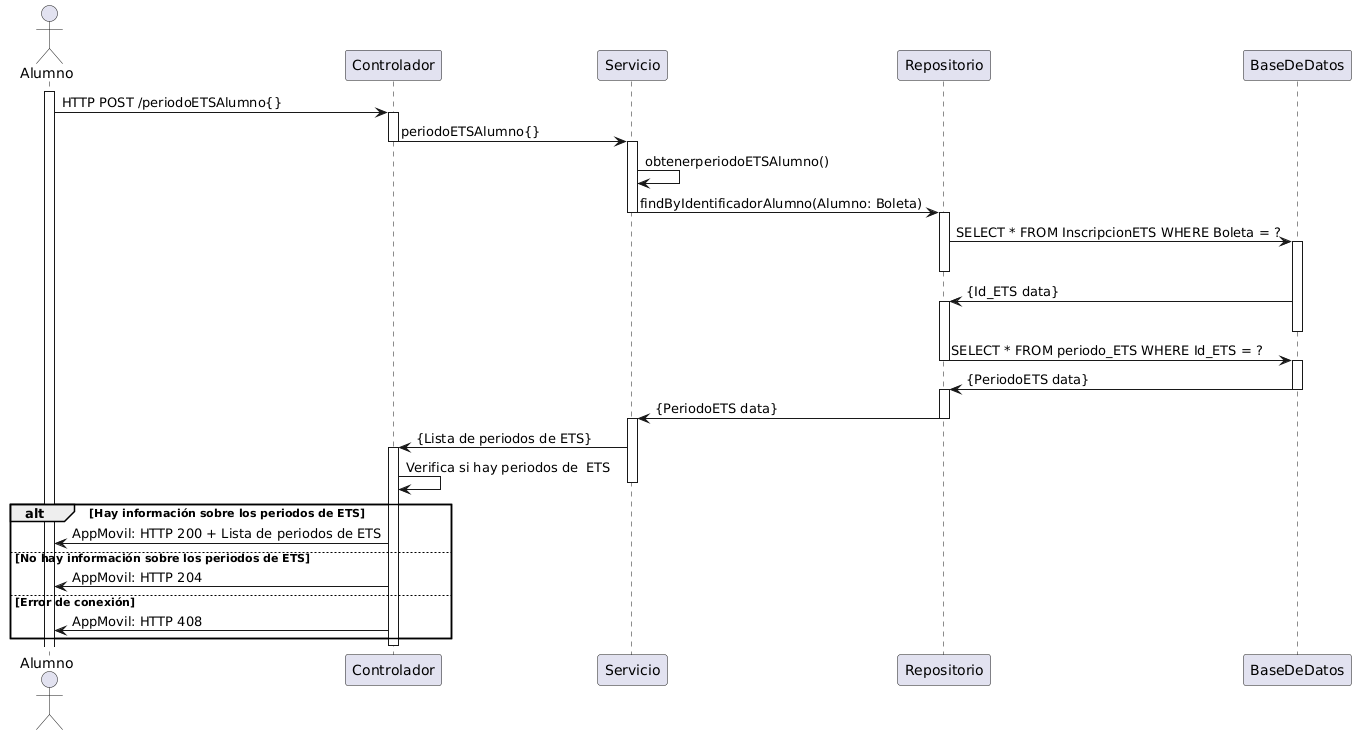
\includegraphics[width=1\textwidth]{Secuencia/CU-16.png}}
		\caption{Diagrama de secuencia del caso de uso número 16 (Consultar periodos de ETS inscritos del alumno).}
		\label{fig:Diagrama de secuencia CU-16}
	\end{center}
\end{figure}

En el diagrama de secuencia \ref{fig:Diagrama de secuencia CU-16} se describe el proceso planeado para el caso de uso \hyperlink{CU-16}{CU-16 Consultar periodos de ETS inscritos del alumno}, mostrando las interacciones que tendrá con la vista, el controlador, el servicio, el repositorio y la base de datos.

\newpage

\subsection{SE-17 Consultar ETS inscritos}

\begin{figure}[htbp!]
	\begin{center}
		\fbox{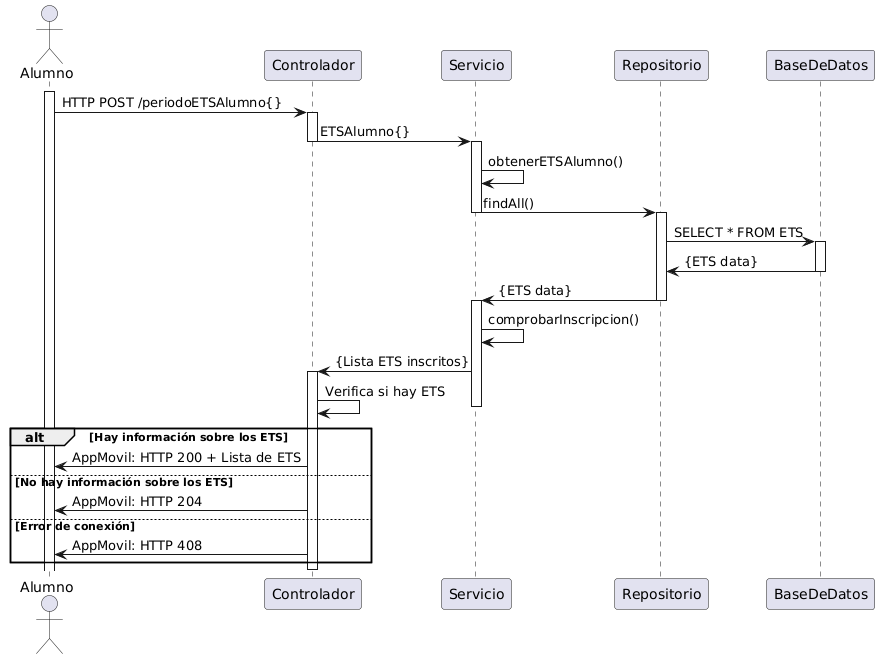
\includegraphics[width=1\textwidth]{Secuencia/CU-17.png}}
		\caption{Diagrama de secuencia del caso de uso número 04 (Consultar ETS inscritos).}
		\label{fig:Diagrama de secuencia CU-17}
	\end{center}
\end{figure}

En el diagrama de secuencia \ref{fig:Diagrama de secuencia CU-17} se describe el proceso planeado para el caso de uso \hyperlink{CU-17}{CU-17 Consultar  ETS inscritos}, mostrando las interacciones que tendrá con la vista, el controlador, el servicio, el repositorio y la base de datos.

\newpage

\subsection{SE-18 Mostrar información del los ETS inscritos}

\begin{figure}[htbp!]
	\begin{center}
		\fbox{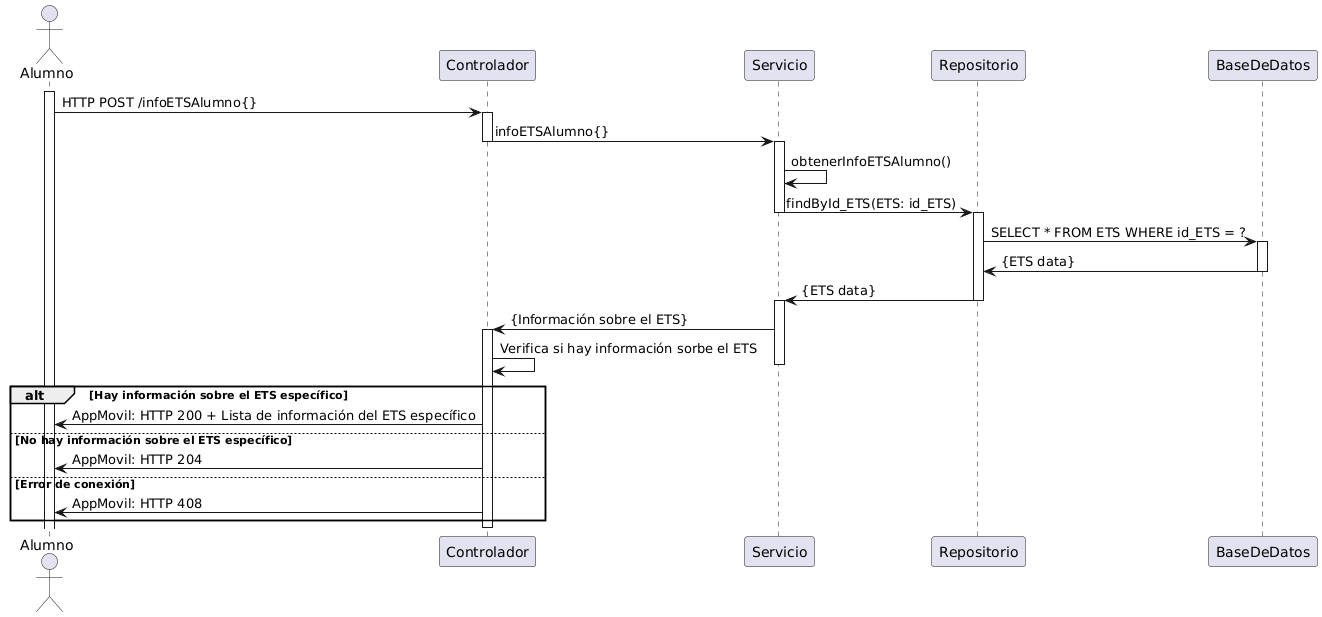
\includegraphics[width=1\textwidth]{Secuencia/CU-18.png}}
		\caption{Diagrama de secuencia del caso de uso número 18 (Mostrar información del los ETS inscritos).}
		\label{fig:Diagrama de secuencia CU-18}
	\end{center}
\end{figure}

En el diagrama de secuencia \ref{fig:Diagrama de secuencia CU-18} se describe el proceso planeado para el caso de uso \hyperlink{CU-18}{CU-18 Mostrar información del los ETS inscritos}, mostrando las interacciones que tendrá con la vista, el controlador, el servicio, el repositorio y la base de datos.

\newpage

\subsection{SE-19 Probar reconocimiento facial}

\begin{figure}[htbp!]
	\begin{center}
		\fbox{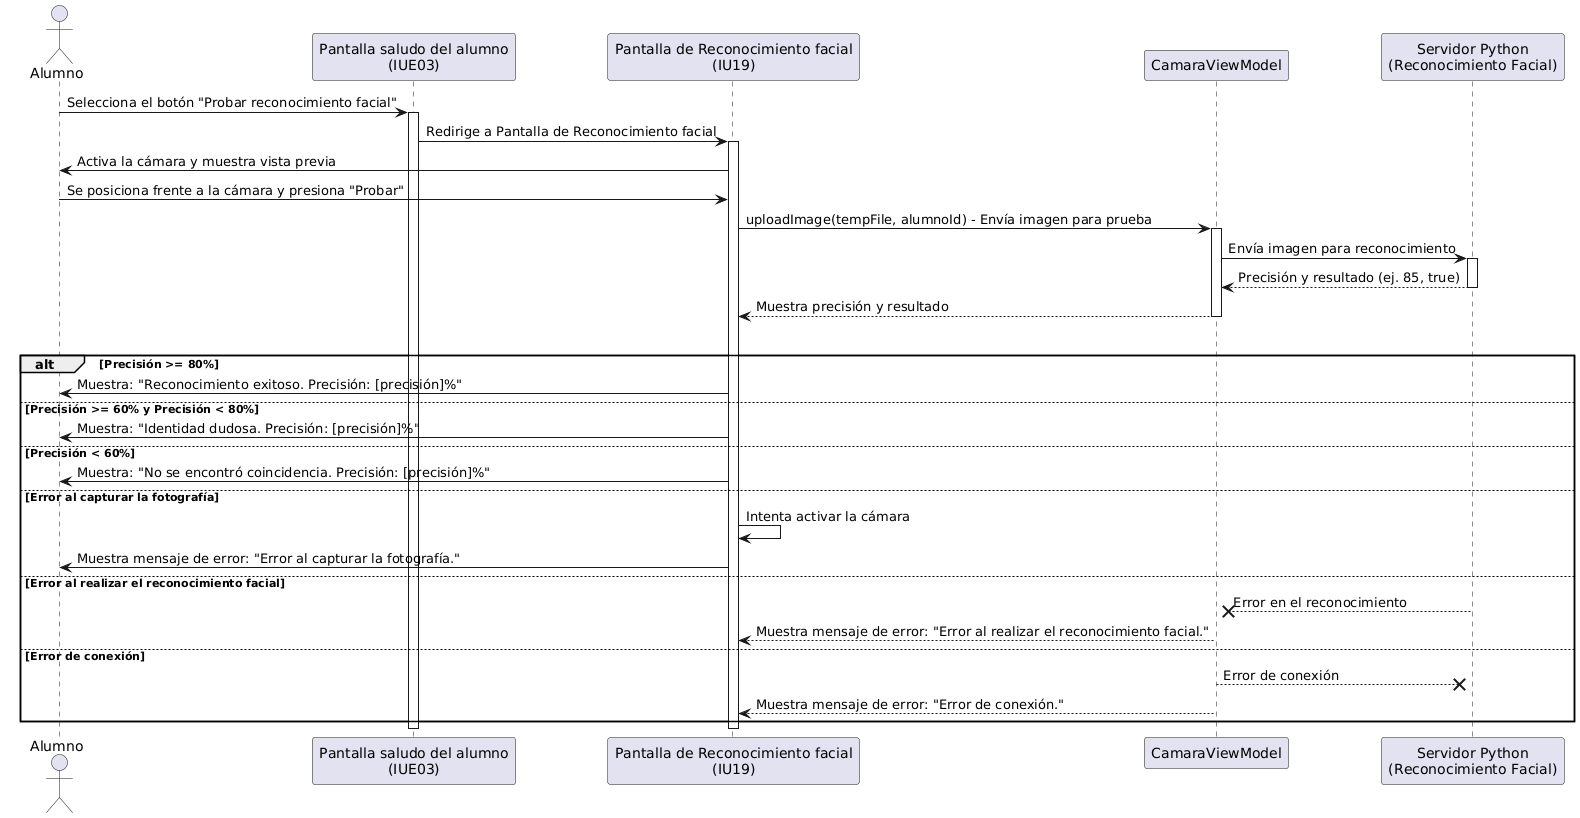
\includegraphics[width=1\textwidth]{Secuencia/CU-19.png}}
		\caption{Diagrama de secuencia del caso de uso número 19 (Probar reconocimiento facial).}
		\label{fig:Diagrama de secuencia CU-19}
	\end{center}
\end{figure}

En el diagrama de secuencia \ref{fig:Diagrama de secuencia CU-19} se describe el proceso planeado para el caso de uso \hyperlink{CU-19}{CU-19 Probar reconocimiento facial}, mostrando las interacciones que tendrá con la vista, el controlador, el servicio, el repositorio y la base de datos.

\newpage

\subsection{SE-20 Revisar información de acceso a los ETS}

\begin{figure}[htbp!]
	\begin{center}
		\fbox{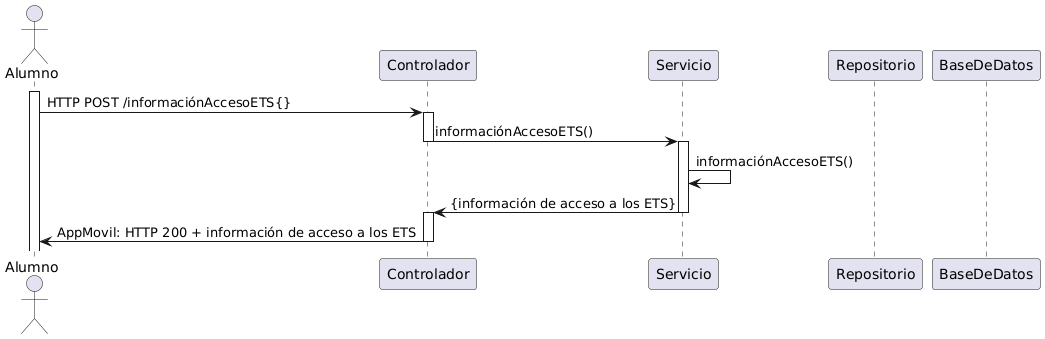
\includegraphics[width=1\textwidth]{Secuencia/CU-20.png}}
		\caption{Diagrama de secuencia del caso de uso número 20 (Revisar información de acceso a los ETS).}
		\label{fig:Diagrama de secuencia CU-20}
	\end{center}
\end{figure}

En el diagrama de secuencia \ref{fig:Diagrama de secuencia CU-20} se describe el proceso planeado para el caso de uso \hyperlink{CU-20}{CU-20 Revisar información de acceso a los ETS}, mostrando las interacciones que tendrá con la vista, el controlador, el servicio, el repositorio y la base de datos.

\newpage

\subsection{SE-21 Dar de alta a alumno}

\begin{figure}[htbp!]
	\begin{center}
		\fbox{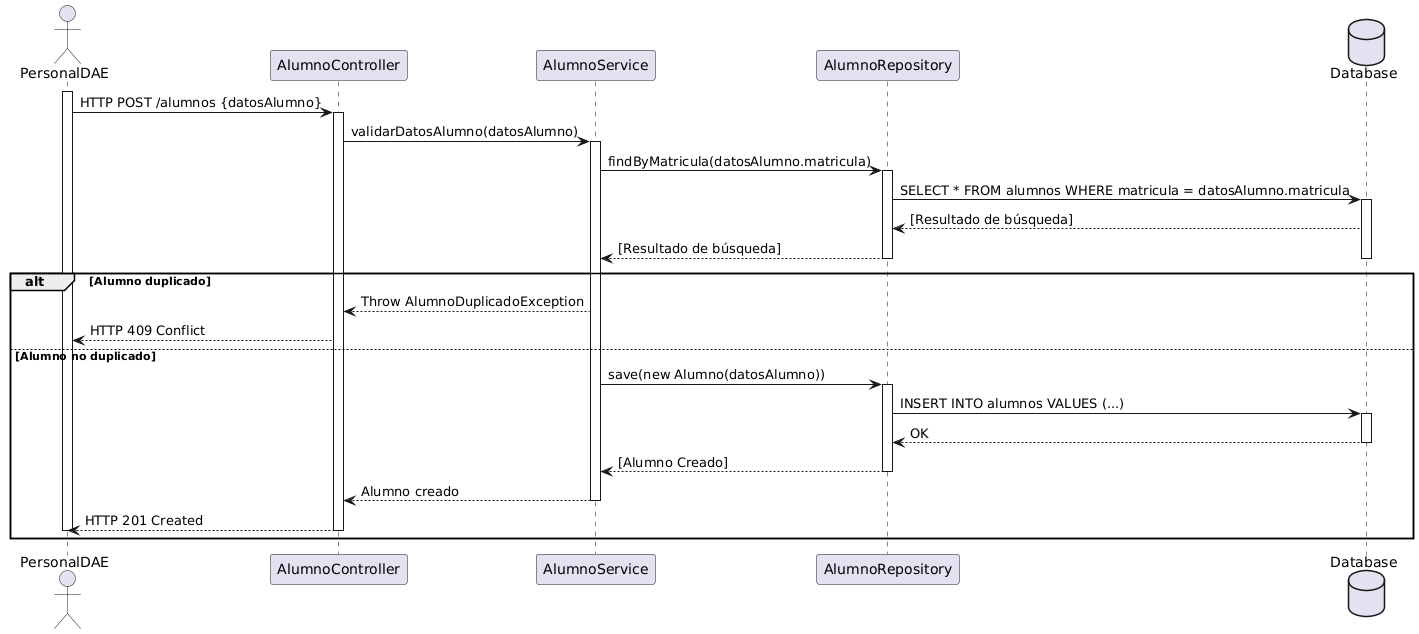
\includegraphics[width=1\textwidth]{Secuencia/CU-21.png}}
		\caption{Diagrama de secuencia del caso de uso número 21 (Dar de alta a alumno).}
		\label{fig:Diagrama de secuencia CU-21}
	\end{center}
\end{figure}

En el diagrama de secuencia \ref{fig:Diagrama de secuencia CU-21} se describe el proceso planeado para el caso de uso \hyperlink{CU-21}{CU-21 Dar de alta a alumno}, mostrando las interacciones que tendrá con la vista, el controlador, el servicio, el repositorio y la base de datos.

\newpage

\subsection{SE-22 Crear credencial y capturar fotografía estudiantil}

\begin{figure}[htbp!]
	\begin{center}
		\fbox{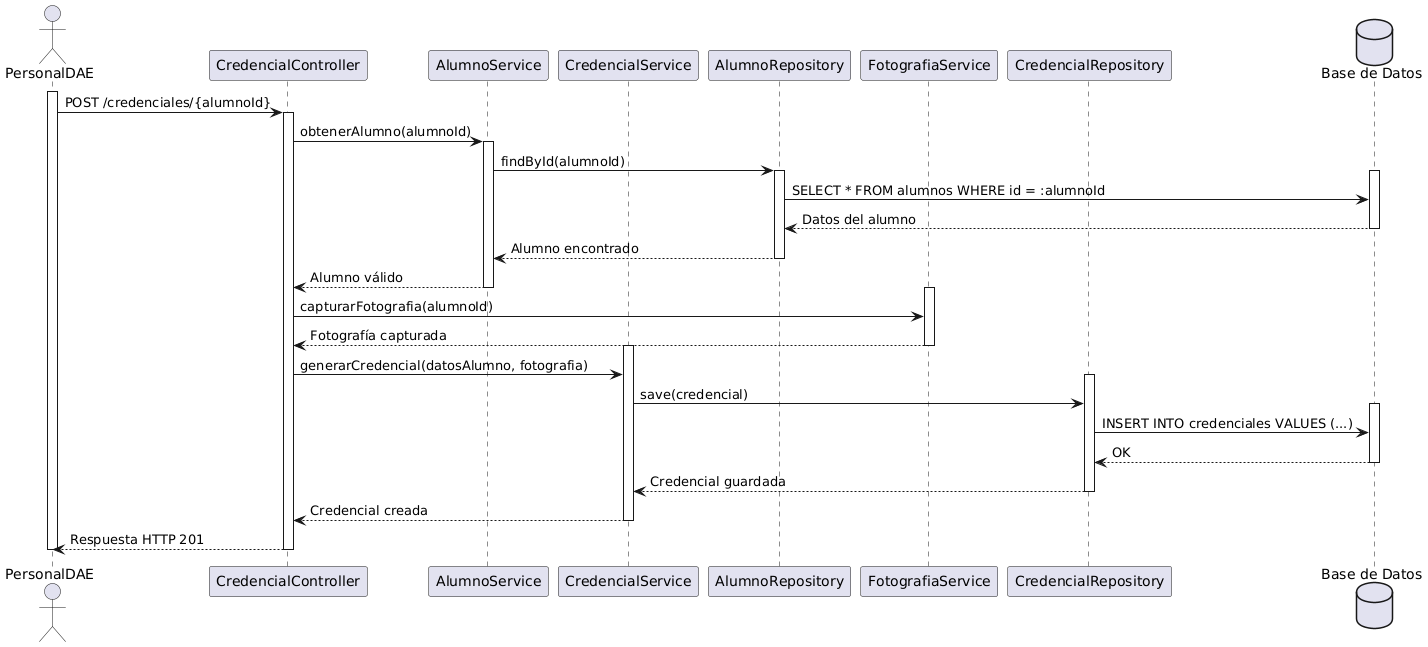
\includegraphics[width=1\textwidth]{Secuencia/CU-22_23.png}}
		\caption{Diagrama de secuencia del caso de uso número 22 y 23 (Crear credencial y capturar fotografía estudiantil).}
		\label{fig:Diagrama de secuencia CU-22 y CU23}
	\end{center}
\end{figure}

En el diagrama de secuencia \ref{fig:Diagrama de secuencia CU-22 y CU23} y se describe el proceso planeado para el caso de uso \hyperlink{CU-22}{CU-22 Crear credencia} y \hyperlink{CU-23}{CU-23 Capturar fotografía estudiantil}, mostrando las interacciones que tendrá con la vista, el controlador, el servicio, el repositorio y la base de datos.

\newpage

\subsection{SE-23 Consultar lista de periodo de ETS}

\begin{figure}[htbp!]
	\begin{center}
		\fbox{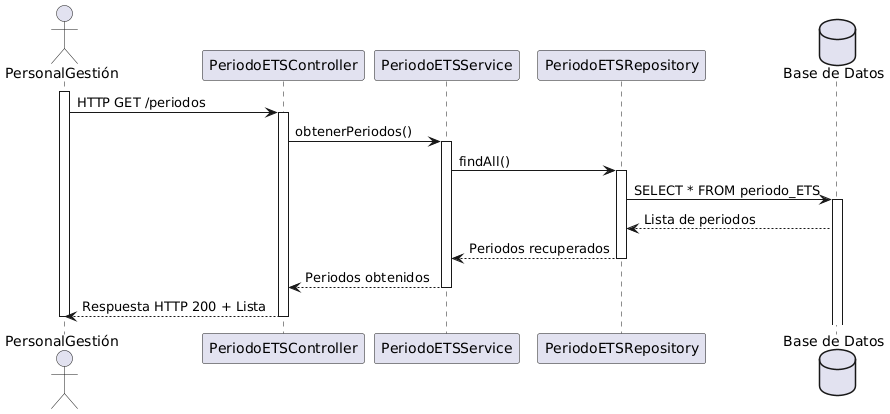
\includegraphics[width=1\textwidth]{Secuencia/CU-24.png}}
		\caption{Diagrama de secuencia del caso de uso número 24 (Consultar lista de periodo de ETS).}
		\label{fig:Diagrama de secuencia CU-24}
	\end{center}
\end{figure}

En el diagrama de secuencia \ref{fig:Diagrama de secuencia CU-24} se describe el proceso planeado para el caso de uso \hyperlink{CU-24}{CU-24 Consultar lista de periodo de ETS}, mostrando las interacciones que tendrá con la vista, el controlador, el servicio, el repositorio y la base de datos.

\newpage

\subsection{SE-24 Dar de alta de periodo de ETS}

\begin{figure}[htbp!]
	\begin{center}
		\fbox{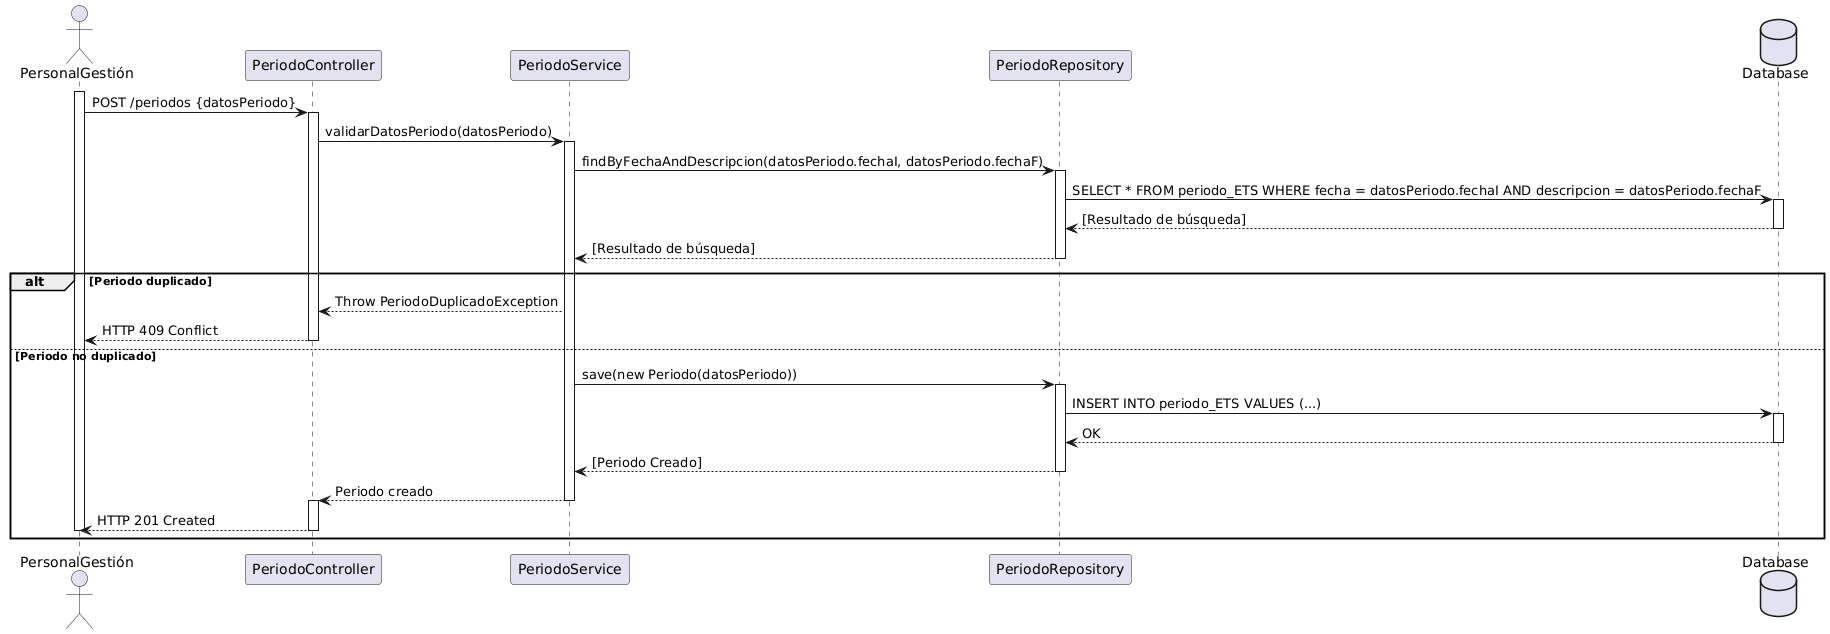
\includegraphics[width=1\textwidth]{Secuencia/CU-25.png}}
		\caption{Diagrama de secuencia del caso de uso número 25 (Dar de alta de periodo de ETS).}
		\label{fig:Diagrama de secuencia CU-25}
	\end{center}
\end{figure}

En el diagrama de secuencia \ref{fig:Diagrama de secuencia CU-25} se describe el proceso planeado para el caso de uso \hyperlink{CU-25}{CU-25 Dar de alta de periodo de ETS}, mostrando las interacciones que tendrá con la vista, el controlador, el servicio, el repositorio y la base de datos.

\newpage

\subsection{SE-25 Consultar lista de ETS}

\begin{figure}[htbp!]
	\begin{center}
		\fbox{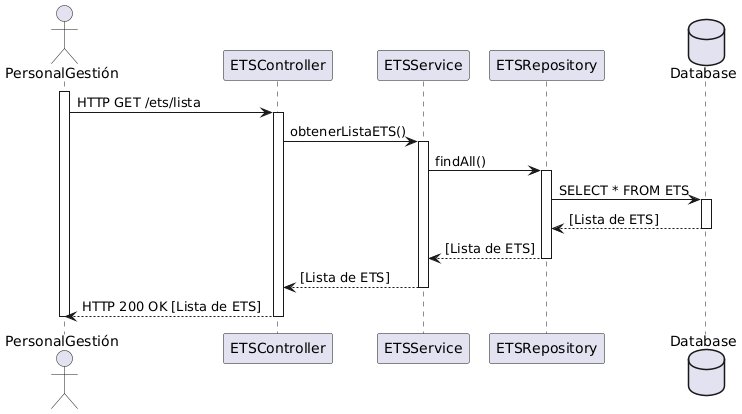
\includegraphics[width=1\textwidth]{Secuencia/CU-28.png}}
		\caption{Diagrama de secuencia del caso de uso número 28 (Consultar lista de ETS).}
		\label{fig:Diagrama de secuencia CU-28}
	\end{center}
\end{figure}

En el diagrama de secuencia \ref{fig:Diagrama de secuencia CU-28} se describe el proceso planeado para el caso de uso \hyperlink{CU-28}{CU-28 Consultar lista de ETS}, mostrando las interacciones que tendrá con la vista, el controlador, el servicio, el repositorio y la base de datos.

\newpage

\subsection{SE-26 Dar de alta ETS}

\begin{figure}[htbp!]
	\begin{center}
		\fbox{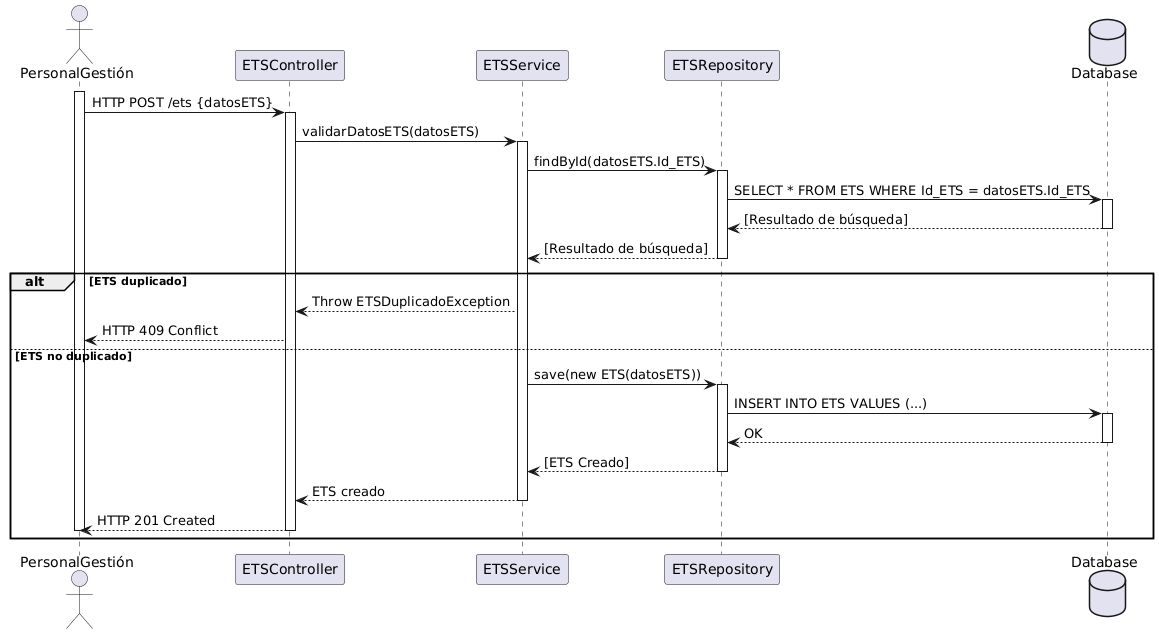
\includegraphics[width=1\textwidth]{Secuencia/CU-29.png}}
		\caption{Diagrama de secuencia del caso de uso número 29 (Dar de alta ETS).}
		\label{fig:Diagrama de secuencia CU-29}
	\end{center}
\end{figure}

En el diagrama de secuencia \ref{fig:Diagrama de secuencia CU-29} se describe el proceso planeado para el caso de uso \hyperlink{CU-29}{CU-29 Dar de alta ETS}, mostrando las interacciones que tendrá con la vista, el controlador, el servicio, el repositorio y la base de datos.

\newpage

\subsection{SE-27 Consultar lista de personal de seguridad}

\begin{figure}[htbp!]
	\begin{center}
		\fbox{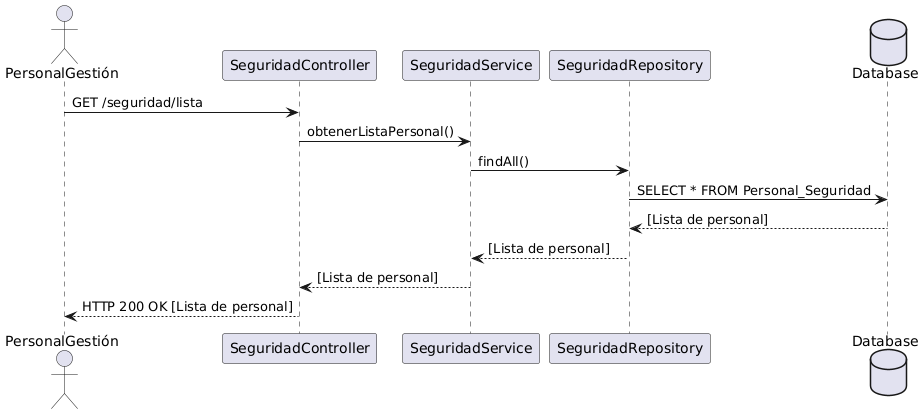
\includegraphics[width=1\textwidth]{Secuencia/CU-32.png}}
		\caption{Diagrama de secuencia del caso de uso número 32 (Consultar lista de personal de seguridad).}
		\label{fig:Diagrama de secuencia CU-32}
	\end{center}
\end{figure}

En el diagrama de secuencia \ref{fig:Diagrama de secuencia CU-32} se describe el proceso planeado para el caso de uso \hyperlink{CU-32}{CU-32 Consultar lista de personal de seguridad}, mostrando las interacciones que tendrá con la vista, el controlador, el servicio, el repositorio y la base de datos.

\newpage

\subsection{SE-28 Dar de alta personal de seguridad}

\begin{figure}[htbp!]
	\begin{center}
		\fbox{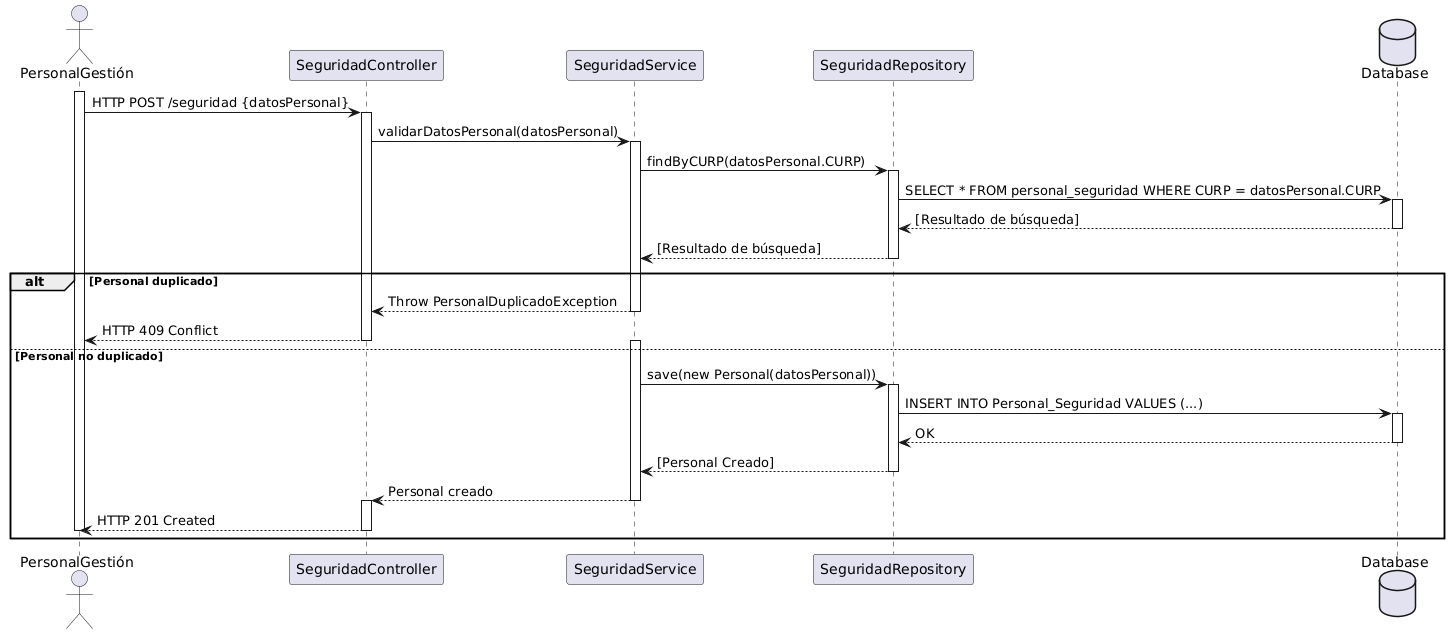
\includegraphics[width=1\textwidth]{Secuencia/CU-33.png}}
		\caption{Diagrama de secuencia del caso de uso número 33 (Dar de alta personal de seguridad).}
		\label{fig:Diagrama de secuencia CU-33}
	\end{center}
\end{figure}

En el diagrama de secuencia \ref{fig:Diagrama de secuencia CU-33} se describe el proceso planeado para el caso de uso \hyperlink{CU-33}{CU-33 Dar de alta personal de seguridad}, mostrando las interacciones que tendrá con la vista, el controlador, el servicio, el repositorio y la base de datos.

\newpage

\subsection{SE-29 Consultar lista de docentes}

\begin{figure}[htbp!]
	\begin{center}
		\fbox{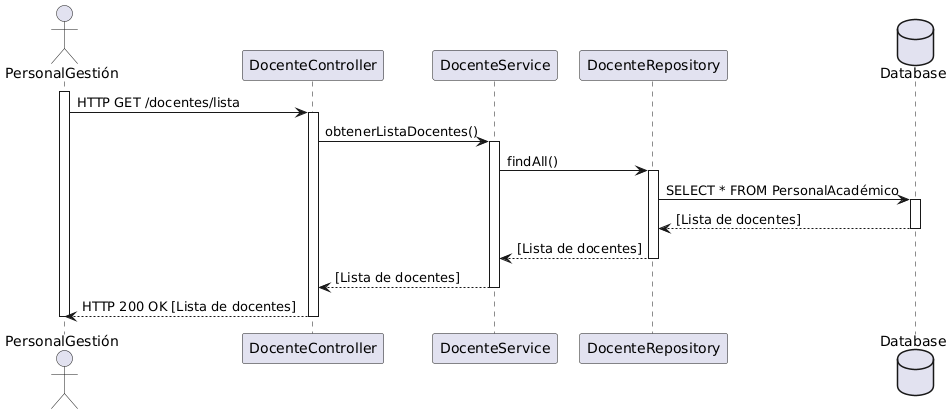
\includegraphics[width=1\textwidth]{Secuencia/CU-36.png}}
		\caption{Diagrama de secuencia del caso de uso número 36 (Consultar lista de docentes).}
		\label{fig:Diagrama de secuencia CU-36}
	\end{center}
\end{figure}

En el diagrama de secuencia \ref{fig:Diagrama de secuencia CU-36} se describe el proceso planeado para el caso de uso \hyperlink{CU-36}{CU-36 Consultar lista de docentes}, mostrando las interacciones que tendrá con la vista, el controlador, el servicio, el repositorio y la base de datos.

\newpage

\subsection{SE-30 Dar de alta docente}

\begin{figure}[htbp!]
	\begin{center}
		\fbox{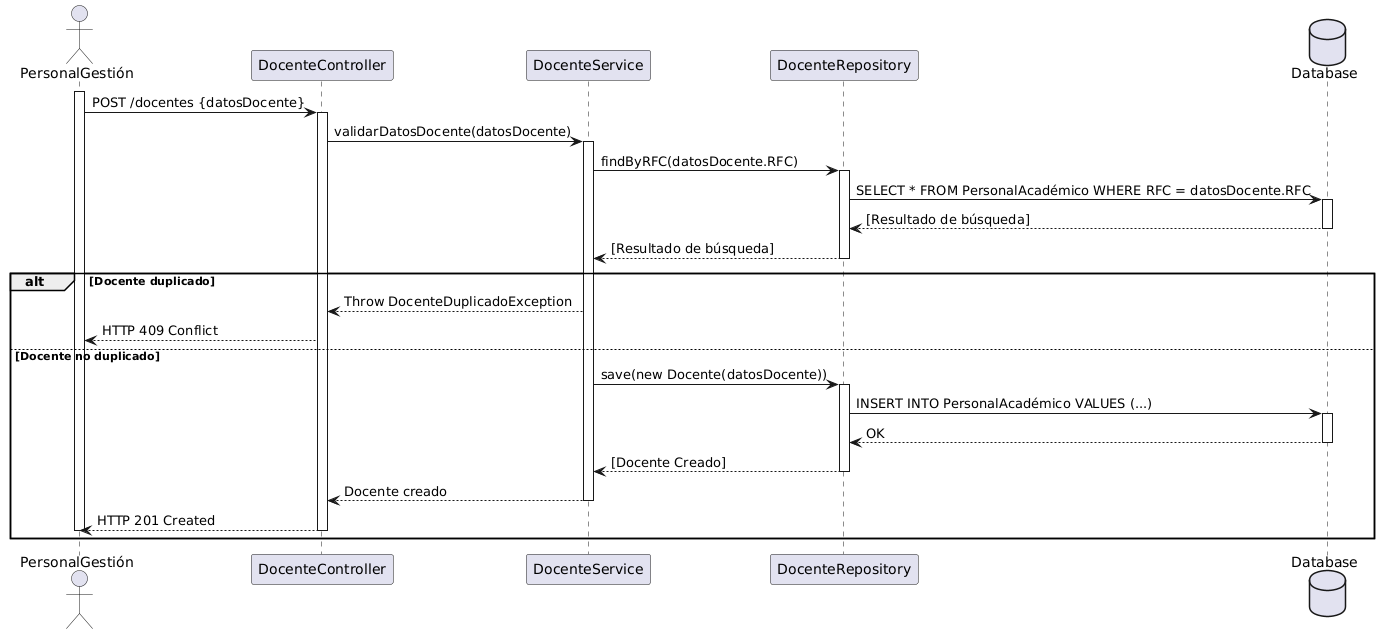
\includegraphics[width=1\textwidth]{Secuencia/CU-37.png}}
		\caption{Diagrama de secuencia del caso de uso número 37 (Dar de alta docente).}
		\label{fig:Diagrama de secuencia CU-37}
	\end{center}
\end{figure}

En el diagrama de secuencia \ref{fig:Diagrama de secuencia CU-37} se describe el proceso planeado para el caso de uso \hyperlink{CU-37}{CU-37 Dar de alta docente}, mostrando las interacciones que tendrá con la vista, el controlador, el servicio, el repositorio y la base de datos.

\newpage

\subsection{SE-31 Solicitar desbloqueo de cuenta}

\begin{figure}[htbp!]
	\begin{center}
		\fbox{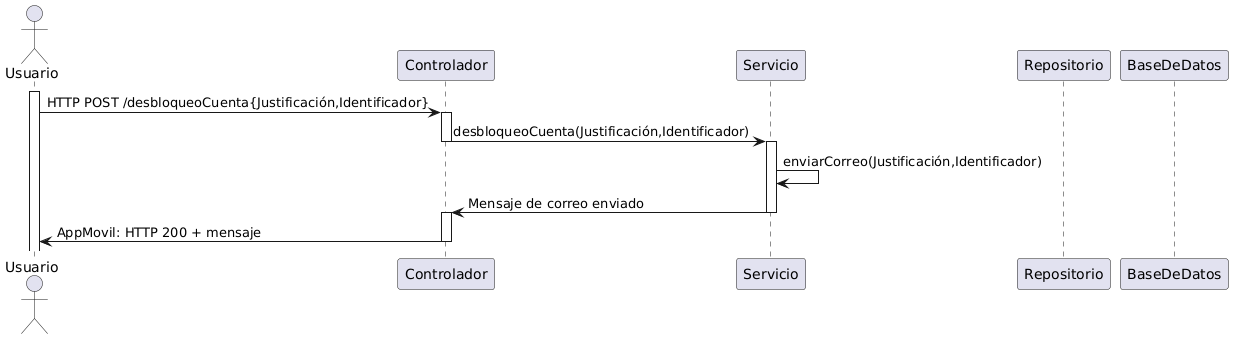
\includegraphics[width=1\textwidth]{Secuencia/CU-40.png}}
		\caption{Diagrama de secuencia del caso de uso número 40 (Solicitar desbloqueo de cuenta).}
		\label{fig:Diagrama de secuencia CU-40}
	\end{center}
\end{figure}

En el diagrama de secuencia \ref{fig:Diagrama de secuencia CU-40} se describe el proceso planeado para el caso de uso \hyperlink{CU-40}{CU-40 Solicitar desbloqueo de cuenta}, mostrando las interacciones que tendrá con la vista, el controlador, el servicio, el repositorio y la base de datos.

\newpage

\subsection{SE-32 Iniciar sesión del sistema web}

\begin{figure}[htbp!]
	\begin{center}
		\fbox{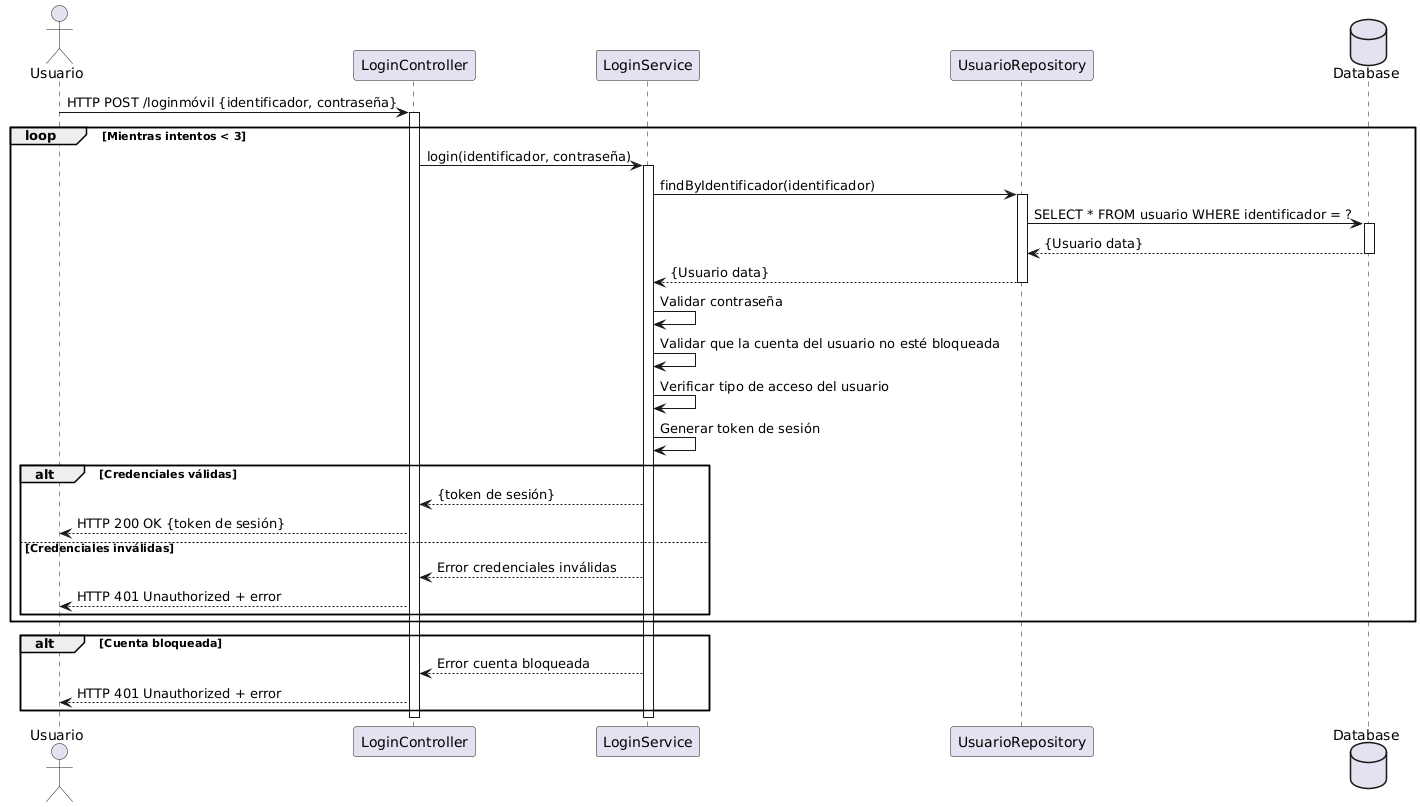
\includegraphics[width=1\textwidth]{Secuencia/CU-41.png}}
		\caption{Diagrama de secuencia del caso de uso número 41 (Iniciar sesión del sistema web).}
		\label{fig:Diagrama de secuencia CU-41}
	\end{center}
\end{figure}


En el diagrama de secuencia \ref{fig:Diagrama de secuencia CU-41} se describe el proceso planeado para el caso de uso \hyperlink{CU-41}{CU-41 Iniciar sesión del sistema web}, mostrando las interacciones que tendrá con la vista, el controlador, el servicio, el repositorio y la base de datos.

\newpage

\subsection{SE-33 Asignar docente de remplazo}

\begin{figure}[htbp!]
	\begin{center}
		\fbox{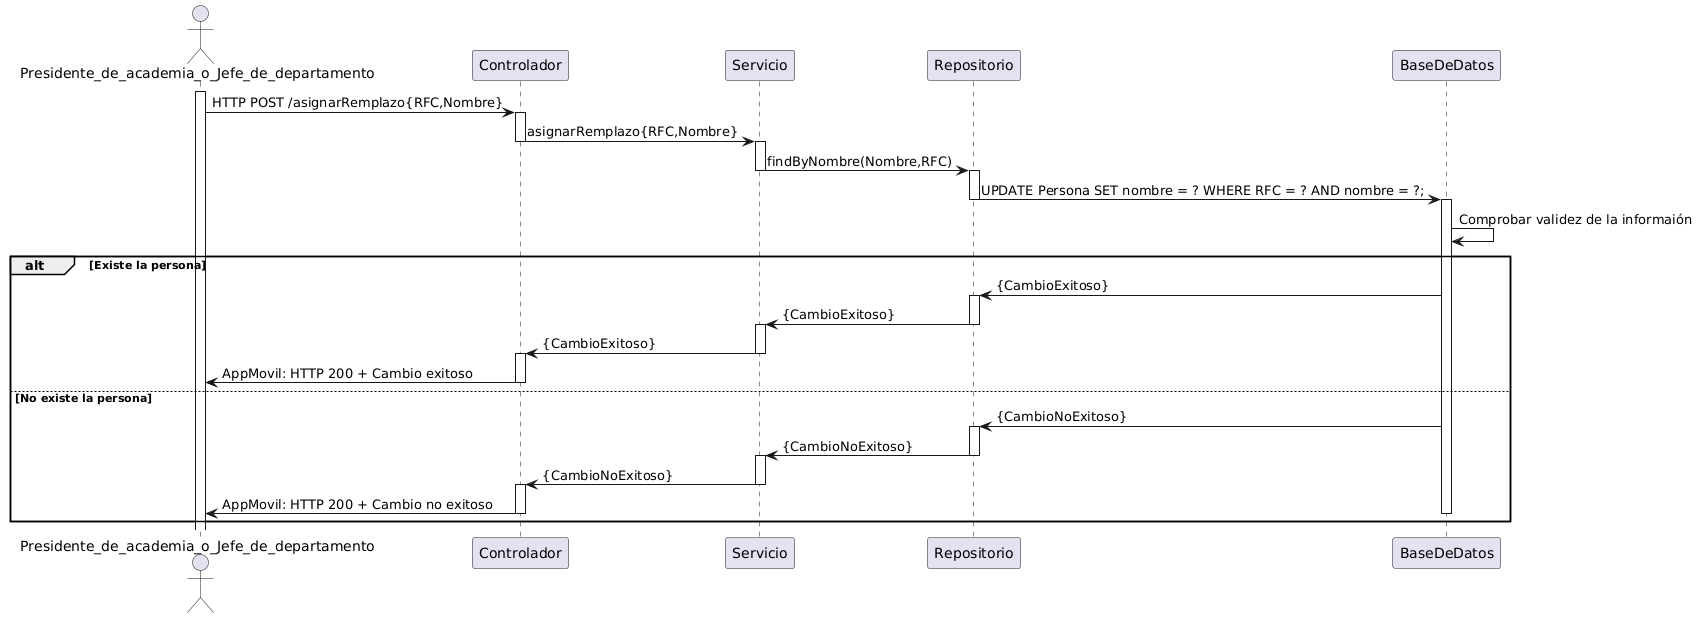
\includegraphics[width=1\textwidth]{Secuencia/CU-42.png}}
		\caption{Diagrama de secuencia del caso de uso número 42 (Asignar docente de remplazo).}
		\label{fig:Diagrama de secuencia CU-42}
	\end{center}
\end{figure}

En el diagrama de secuencia \ref{fig:Diagrama de secuencia CU-42} se describe el proceso planeado para el caso de uso \hyperlink{CU-42}{CU-42 Asignar docente de remplazo}, mostrando las interacciones que tendrá con la vista, el controlador, el servicio, el repositorio y la base de datos.